\documentclass{UoNMCHA}
\usepackage[authoryear]{natbib}
\usepackage{array,booktabs} % For nice tables
\usepackage{amsmath,amsfonts,amssymb} % For nice maths
\usepackage{color,mathtools}
\usepackage{enumerate,tensor}
\usepackage{listings}
\usepackage{subfig}
\usepackage{multicol}
\usepackage{hyperref}
\usepackage{float}
\usepackage[dvipsnames]{xcolor}
\usepackage[mathscr]{euscript}
\usepackage[parfill]{parskip}   % For replacing paragraph indenting with a newline instead
\usepackage{enumitem}
\usepackage[tableposition=top]{caption}

% Number equations per section
\numberwithin{equation}{section}

\hypersetup{
%    bookmarks=true,         % show bookmarks bar?
%    unicode=false,          % non-Latin characters in AcrobatÕs bookmarks
%    pdftoolbar=true,        % show AcrobatÕs toolbar?
%    pdfmenubar=true,        % show AcrobatÕs menu?
%    pdffitwindow=false,     % window fit to page when opened
%    pdfstartview={FitH},    % fits the width of the page to the window
%    pdftitle={My title},    % title
%    pdfauthor={Author},     % author
%    pdfsubject={Subject},   % subject of the document
%    pdfcreator={Creator},   % creator of the document
%    pdfproducer={Producer}, % producer of the document
%    pdfkeywords={keyword1} {key2} {key3}, % list of keywords
%    pdfnewwindow=true,      % links in new window
    colorlinks=true,       % false: boxed links; true: colored links
    linkcolor=blue,          % color of internal links
    citecolor=blue,        % color of links to bibliography
%    filecolor=magenta,      % color of file links
    urlcolor=blue           % color of external links
}

\definecolor{MATLABKeyword}{rgb}{0,0,1}
\definecolor{MATLABComment}{rgb}{0.1328125,0.54296875,0.1328125}
\definecolor{MATLABString}{rgb}{0.625,0.125,0.9375}

\lstset{language=Matlab,
    basicstyle=\small\ttfamily,
    keywordstyle=\color{MATLABKeyword},
    %identifierstyle=,
    commentstyle=\color{MATLABComment},
    stringstyle=\color{MATLABString},
    numberstyle=\tiny,
    %numbers=left,
    basewidth=0.5em}

\firstpage{1}    % Set page number for first page
\UoNMCHAreportNo{Final Year Project} %Report number
\UoNMCHAyear{2019}   % Year\\
\shorttitle{Beam type 3D Printer} %For odd pages
%%%%%%%%%%%%%%%%%%%%%%%%%%%%%%%%%%%%%%%%%%%%%%%%%%%%
\begin{document}
\title{Beam type 3D Printer \\ \ \\
{\small MECH4841 Final Year Project Report  \\\textcolor{red}{July 2020}}}
\author[UoNMCHA]{Abid Khan}
\address[UoNMCHA]{
Student of Mechatronics Engineering,\\
The University of Newcastle, Callaghan, NSW 2308, AUSTRALIA \\
Student Number: \textcolor{red}{c325555} \\
E-mail: \href{mailto:Abid.Khan@uon.edu.au}{\textsf{Muhammad.H.Khan@uon.edu.au}}}
%%%%%%%%%%%%%%%%%%%%%%%%%%%%%%%%%%%
\maketitle
\onecolumn

%%%%%%%%%%%%%%%%%%%%%%%%%%%%%%%%%%%%
\vspace{-5mm}
\section*{Dot Point Summary}
%\vspace{mm}

This project explores:
\begin{itemize}
	\color{red}
	\item Modelling and controlling a robotic manipulator
	\item Camera modelling and feature point extraction
	\item Training a machine learning based object detector
	\item Deriving a visual-servoing controller 


\end{itemize}

\newpage
\vspace{-5mm}
\section*{Abstract}

This report covers the design aspect of a tower crane-based 3D printer. It includes the energy based mathematical modelling the dynamics of a fully actuated system using Euler-Lagrange equations of motions. The system consists of one rotational and three prismatic joints. It also covers the forward in inverse kinematics for the project along with two control designs which is linear quadratic regulator and model predictive control. It also covers a way for generating a trajectory with constraints and slew rate limits. This report will discuss the results produced by the simulations of the two control designs. \\
The future work for this project would be the implementation all the control actions on the hardware and compared with the traditional gantry-based 3D printer hardware.


%%%%%%%%%%%%%%
\newpage
\vspace{-2mm}
\section*{Acknowledgements}

Dr Alejandro Donaire has provided significant amount of help and support with this project. He is also the supervisor for this project. I’d also like to thank my family and friends for providing the support and stability I needed for the successful completion of this report. Some of those friends are listed below.
\begin{itemize}
	\item Bill McBride for his faith.
	\item Patrick Harper for his help.
	\item Muhammad Hasham for his help.
	\item Paul Hughes for his help.
	
\end{itemize}

%%%%%%%%%%%%%%%%%%%%%%%%%%%%%
\newpage
\tableofcontents
\listoffigures
\listoftables
\newpage
%%%%%%%%%%%%%%%%%%%%%%%%%%%%%%%
\section*{Chapter 1}
\addcontentsline{toc}{section}{Chapter 1}
\section{Introduction}

The project aims at design and simulation of a 3D printer for house construction. The project is focused on the modelling, analysis, simulation and control and evaluation of a rotational machine with prismatic arm, the 3D printer, that moves in its workspace where the walls of the house are to be printed. An active counterweight balancing system is attached to the printer to increase the precision, stability and speed of the machine. This report will also work on comparing different controllers to find the appropriate solution for the project.

    
%%%%%%%%%%%%%%%%%%%%%%%%%%%%%%%%    
\section{Problem Formulation}\label{Problem Formulation}

\subsection{Use of 3D printing for houses}\label{Use of 3D printing for houses}
    
\subsection*{Previous design – full frame design}
Traditionally, 3D printers use a gantry-based design which operate by following a precomputed path and extruding a layer of material upon a work-surface for multiple layers to create a desired object. This filament is extruded out through a nozzle, whose movement is precisely controlled by a computer which operates motors that slide the nozzle along the X gantry, the X gantry in Y gantry and both gantries along the Z gantry. 

\begin{figure}[H]
	\begin{center}
		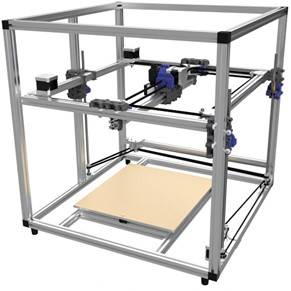
\includegraphics[width=.5\linewidth]{figs/Picture1}
		\caption{A  common 3 axis cartesian FDM 3D printer commonly consisting of 3 actuators}
		\label{figs/Picture1}
	\end{center}
\end{figure}
	
This framework has been applied by Fused Deposition Modelling (FDM) 3D printers and has shown promising results.
However, this method has few limitations:

\begin{itemize}
	\item Size of the gantry system required increases dramatically when considering the construction of larger buildings (it must be larger than the building to fully encompass it).
	\item Construction industry is a very conservative market that is slow to change. It would be easier to use a system that is tried and tested in a construction environment.
	\item Due to the bulky structure require it to be disassembled For transportation purposes.
	
\end{itemize}

Therefore, a methodology to use tower cranes to perform 3-D printing was proposed.

\subsection*{Use of tower crane design}

Jerry rig previously robustly designed systems \\
Currently not used as this hasn’t been applied to this problem \\
Precision \\

\subsection{In-scope} \label{In-scope}

\begin{itemize}
	\item Modelling Tower Crane.
	\item Controlling Tower Crane.
\end{itemize}

\subsection{Out-of-scope} \label{Out-of-scope}

\begin{itemize}
	\item Proof of concept – Friction and damping were not considered.
	\item Assumed perfect motors with output and slew rate limits .
	\item Assumed perfect encoders and thus perfect state estimation – no observer or state estimation considered.
	
\end{itemize}
	
\subsection{Crane Systems} \label{Crane Systems}

What does a crane look like? (insert picture)\\
How do cranes work? (counterbalance ect)\\
Use of cranes in construction \\
Humans get tired \\
Mistakes happen\\
Humans require food\\ 
Humans cant get whipped without quitting\\
Robots cant unionise \\

\subsection{Safety Considerations} \label{Safety Considerations}

Can you prevent over-swinging? Oscollations in control are dangerous for cranes, does this mean we need smart control algorythms
Moments balancing 

\section{Additive Manufacturing}\label{Additive Manufacturing}

Additive manufacturing (AM) sometimes also known as Additive Layer Manufacturing (ALM) is a term that is commonly used in industries for 3D printing. In general, it is a process controlled by computer by depositing material usually in layers. There are a number of various AM processes some of which include Binding Jetting, Direct Energy Deposition, Material Extrusion, Powder Bed Fusion, Sheet Lamination, Vat Polymerization and Wire Arc Additive Manufacturing. \\

Hideo Kodama of Nagoya Municipal Industrial Research Institute was one of the earliest to invent 3D printing manufacturing equipment, he invented two additive methods for fabricating 3D models. There are many materials that are currently used such as biochemicals, ceramics metals, thermo plastics and specialised concrete. AM is used across a growing number of industries creating a wide range of products, some of these industries include aerospace, automotive, construction and medical. \\

AM was initially considered to be only used for rapid prototyping however the increase in precision and repeatability has led it to be used in everyday manufacturing This is due to cheaper material availability and greater support and machines availability in the market. There are significant advantages that can be achieved from this process which includes printing hollow and complex structures. \\

The reason for proposing this project is to build an AM machine that could print houses. which in turn would lower environmental footprint (How does it lower environmental footprint?) while also providing cheaper housing solution.  By minimising the use of material as these structures can be printed hollow it will also benefit people living in areas where wood and other raw materials are scarce. Since this is a relatively new process there are still ways these things can be improved one of the reason is to transport a bulky Machine to build houses. (Add something about being able to build complex structures) this Issue can be resolved by using a beam type 3D printer and to have a counterbalancing mechanism for increased stability. \\

With the advancements in composite materials like concrete, special additives can be added to concrete to set it in mere minutes which used to be days. This will advance the construction process to be completed in a matter of days rather than a few months. This will not only reduce the cost of the construction significantly but also delivered the houses faster, in order to achieve this, a control system for a beam type 3D printer needs to be made.

\section{Automation for Precision manufacturing}\label{Automation for Precision manufacturing}

In the modern days, the manufacturers are pushing for tighter tolerances faster turnarounds and cheaper components. This has led to the use of advanced automation in wide spread applications in an increasing number of industries. This not only increases parts repeatability in micro or ultra precision machining processes, this also significantly reduces the labour required to produce a part this in turn results in a per piece cost reduction specially in higher volume applications. This also insulates the customer against future price volatility due to labour market. Some common implementations of control theory in this context are Automated lathes; CNC machines and 3D printing devices. \\

It is control theory that allows to control of dynamical systems in various engineered processes using machines. The objective is to make a control system that enables us to make precisely coordinated control actions that optimise tool pathing, reduce delay, overshoot and ensuring ensure control stability. The controller that works by minimising the difference between desired value and the actual value is called error which is applied as feedback to initiate a control action which works intuitively to reduce the value between desired and actual value. \\

Control theory allows us to achieve repeatability even when faced with a nonlinear or highly complex system. 

\section{Dynamic Systems}\label{Dynamic Systems}

Before proceeding, it is important to know what dynamic systems are. A system whose current state produces its following state by a certain principle of change and thus produces a trajectory in state space is called a dynamic system. Consider a system where the derivative of the states is a function of the states only:

\begin{equation} \label{state equation}
\dot{x} = f(x)
\end{equation} 

Equation \ref{state equation} represents an autonomous dynamic system as the next state is a function of the current state. Successive application of this expression generates a sequence: From \colorbox{red}{(Khalil, 2002)}

\begin{equation} \label{arrows equation}
\dot{x}=f\left(x\right)\rightarrow\ddot{x}=f\left(\dot{x}\right)\rightarrow\dddot{x}=f\left(\ddot{x}\right)\rightarrow\ldots
\end{equation} \\

This sequence can be as long or short as one wishes but an important form of change in the system is the zero change where the rate of change in the states becomes zero i.e., stability, where the dynamics actively recreate the preceding state into current state. This means that for a certain equilibrium point $x_{c}= 0$, the function $f(x_{c})=0$. The equilibrium point can be stable or unstable, the criterion for is explained below. From \colorbox{red}{(Khalil, 2002)} \\

The equilibrium point of the system is: \\

\begin{itemize}
	\item 	Stable if, for each $\epsilon>0$ there is a $\delta=\delta (\epsilon)>0$ such that,
	\begin{equation*}
		\left|\left|x\left(0\right)\right|\right|<\delta\rightarrow x(t)<\epsilon,\forall t>0  
	\end{equation*}
 	\item Unstable if it is not stable.
 	\item Asymptotically stable if it is stable and $\delta$ can be chosen such that,
	\begin{equation*}
	\left|\left|x\left(0\right)\right|\right|<\delta=>\lim_{t\to \infty}{x(t)=0}
	\end{equation*}
	
\end{itemize}

\section{State Space Models}\label{State Space Models}

A model that represents a physical system using its inputs, outputs and states as variables related to each other by a set of differential equations is called a state space model. The states of the system can evolve with time depending on their current values or the values of inputs introduced into the system over time. The states of the system can be represented as vectors in a confined space. The state space model is dependent on the type of system that we are dealing with. Generally, all physical systems are characterized into linear or non-linear systems, both of which are explained briefly in the next section.


\section{Linear and Non-Linear Systems}\label{Linear and Non-Linear Systems}

The most general form of a dynamic system of n state variables is usually defined by an equation expressing the time derivative of the state variables as a function of time, t, the state variables, $x_1\mathrm{,\ }x_2, …, x_n$ and input variables $u_1\mathrm{,\ }u_2, …, u_m$. With $x=\left[x_1\mathrm{\ } x_2\mathrm{\ } \ldots\mathrm{\ } x_n\right]^\mathrm{T}$, $u=\left[u_1\mathrm{\ } u_2\mathrm{\ } \ldots\mathrm{\ } u_m\right]^\mathrm{T}$, it may be written. 

\begin{equation}
	\mathbf{\dot{x}=f(t,x,u)}
\end{equation}

Many systems do not have input variables, or they may be written as functions of the time and state variables. One class of such functions are \underline{linear systems} which have the form:

\begin{equation}
\mathbf{\dot{x}=Ax}
\end{equation}

where $A=\left[a_{ij}(t)\right]$ is an $n\times n$ matrix of time dependent functions. Solutions to such a system have the property that any linear combination of solutions is itself a solution. They form a vector space, the state space. The constant vector function $x_0=0$ is always a member of the state space. It has the property that ${\dot{x}}_0=0$ and is an equilibrium state of the system.


When each of the $a_{ij}$ are constant, the general solution to the system usually has the form: 

\begin{equation}
\mathbf{\dot{x}=Be}
\end{equation}

Here $\mathbf{e}$ is a vector, $\left[e_1\mathrm{(t)\ } e_2\mathrm{(t)\ } \ldots\mathrm{\ } e_n\mathrm{(t)} \right]^\mathrm{T}$, of time dependent functions where  $e_i\left(t\right)=e^{\lambda_it}$ and $\mathbf{B}$ an $n\times n$ matrix of constants. The $\lambda_i$ are the eigen values of $\mathbf{A}$ which may be complex. The real part gives rise to an exponential function, the complex part is associated with a sinusoidal function.  Any state is a linear combination of some, not necessarily all, of the functions in\ $\mathbf{e}$. The behaviour of a state over time depends on the sign of the real parts of the eigenvalues contributing to the state:

\begin{itemize}
\item	If any sign is positive, the size of the state grows exponentially. This is an unstable state.

\item	If no sign is positive but at least one associated eigenvalue has real part 0, the associated function in $\mathbf{e}$ is purely sinusoidal or constant. If the state starts close to the equilibrium state, $\mathbf{x}_\mathbf{0}$, it will stay close to equilibrium over time. The state is stable.

\item	If all signs are negative, the state will be dominated by exponential decay and the state will tend towards the equilibrium state, $\mathbf{x}_\mathbf{0}$. The state is asymptotically stable.
\end{itemize}

Most realistic dynamic systems are far more complex than linear systems entailing algebraic combinations of power, sinusoidal, exponential, and other nasty functions of the time and state variables. Analytic solutions are usually impossible and numerical methods must be employed. But the notions of stability carry over to these problems and it is often possible to decide when they give rise to stable and asymptotically stable solutions.


\section{Energy Based Modelling}\label{Energy Based Modelling}

The dynamic equations of any mechanical system are obtainable from the renowned Newtonian classical mechanics. The disadvantage of this formalism is the usage of the variables in vector form, complicating substantially the analysis when increasing the joints or if there are rotations present in the system. In these situations, it is favourable to utilize the Lagrange equations, which have a formalism of scale, simplifying the analysis for any mechanical system. To use Lagrange equations, it is essential to follow four steps listed below:

\begin{itemize}
\item Calculation of all kinetic energies.
\item Calculation of all potential energies.
\item Calculation of the Lagrangian.
\item Solve the equations.

\end{itemize}

Where the kinetic energy can be both translational and rotational, this form of energy can be a function of both, position, and the velocity $K(q(t), q(t))$. \\
The potential energy is due to conservative forces such as the forces exerted by gravity and springs, this energy is in terms of the position $U(q(t))$. \\
Is defined the Lagrangian as

\begin{equation}
	\mathbf{L}\ =\ \mathbf{K}\ – U
\end{equation}

Therefore, the Lagrangian is defined of the following in general terms.

\begin{equation}
\mathbf{L}\left(\dot{\mathbf{q}},\mathbf{q}\right)=\mathbf{K}^\ast\left(\mathbf{q},\dot{\mathbf{q}}\right)-\mathbf{U}\left(\mathbf{q}\right)
\end{equation}

Finally, the Euler-Lagrange equations of motion for a system of i degree of freedom are defined as follows. **********************

\begin{equation}
\mathbf{L}\left(\dot{\mathbf{q}},\mathbf{q}\right)=\mathbf{K}^\ast\left(\mathbf{q},\dot{\mathbf{q}}\right)-\mathbf{U}\left(\mathbf{q}\right)
\end{equation}


Where $i=1,\ldots,n,\tau_i$ are the forces or pairs exerted externally in each joint, besides nonconservative forces such as friction, resistance to movement of an object within a fluid and generally those that depend on time or speed. It will be obtained an equal number of dynamic equations and DOF. \textcolor{red}{(Duarte Madrid, Henao and Querubín, 2017)}

\section{Kinematics}

A precise definition of kinematics is found on Oxford dictionary which states, “Kinematics is a branch of mechanics concerned with the motion of objects without reference to the forces which cause the motion”. Kinematics. (2020). In Oxford Online Dictionary 

\subsection{Forward Kinematics}

Forward kinematics is a process of calculating end effector’s position and velocity by using known joint angles and displacements. While it is mostly used for an end effector position it could also be used for any frame in space with respect to a reference.

\subsection*{Denavit Hartenberg}
As the name prescribes, Denavit Hartenberg convention was introduced by Jacques Denavit and Richard Hartenberg in 1955.The purpose of this convention was to standardise the coordinate frames for spatial linkages. The term Denavit Hartenberg is widely known in the engineering fields. \\

There are four parameters associated with this convention. This technique is used for attaching reference frames to the links of a robotic manipulator or kinematic chains.

\begin{figure}[H]
	\begin{center}
		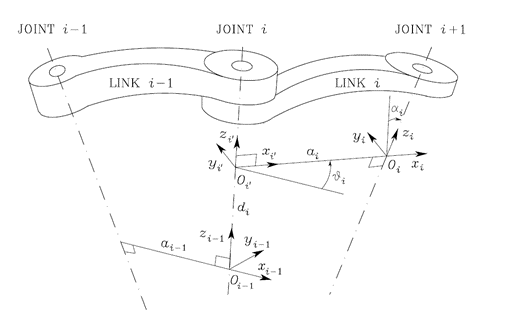
\includegraphics[width=.5\linewidth]{figs/Picture2}
		\caption{A  common 3 axis cartesian FDM 3D printer commonly consisting of 3 actuators}
		\label{figs/Picture2}
	\end{center}
\end{figure}

With those four parameters, coordinates can be translated from $O_{i-1}X_{i-1}Y_{i-1}Z_{i-1}$ to $O_iX_iY_iZ_i$.

$\mathbf{d}$: offset along previous z to the common normal \\
$\mathbf{\theta}$: angle about previous z, from old x to new x\\
$\mathbf{r}$: length of the common normal (aka a, but if using this notation, do not confuse with $\alpha$ ). Assuming a revolute joint, this is the radius about previous z.\\
$\mathbf{\alpha}$: angle about common normal, from old z axis to new z axis\\

**********************

\begin{equation}
\mathbf{L}\left(\dot{\mathbf{q}},\mathbf{q}\right)=\mathbf{K}^\ast\left(\mathbf{q},\dot{\mathbf{q}}\right)-\mathbf{U}\left(\mathbf{q}\right)
\end{equation}

***********************

By using the matrix above a homogenous transformation matrix is produced where R is a 3x3 rotation submatrix and T is a 3x1 translational vector. 

\subsection{Inverse Kinematics}

Inverse kinematics is a processed for determining a value of the joint variable given the position and orientation of an end effector. The problem of inverse kinematic can be solved analytically for some simple manipulators utilising algebraic intuition. The problem can become complex when dealing with nonlinearities. In these cases, there may exist multiple (finite or infinite), unique or no solutions. \\

A modern method to solve an inverse kinematic problem is to pose the question as a numeric optimization problem. In many solvers, it is convenient to use a non-negative, balanced solution to prevent any one element from overfitting. In this case we can leverage scalar quadratic cost functions. \\

Given a set of joint angles (q), the quadradic state error  x–xe can be concatenated through a scaling matrix K. We can pose this in common Sequential Quadratic Programming SQP solutions as a total cost. We can also minimize the deviation q from zero with a scaling factor W. A minimal solution to these implies minimum end effector error and minimum deviation from joint space.  \\


\begin{gather*}
	\left(q^\star,x^\star\right)=\arg{\min \lim_{q,x}{q^{T}W}q}+\left(x-x_e\right)^\top K\left(x-x_e\right) \\
	\mathrm{\ s.t.\ }x-k\left(q\right)=0
\end{gather*}

given the current configuration and pose the above can be initialised. (Renton, n.d.)
For the purposes of this project simple trigonometric coordinate transformations between cartesian and cylindrical coordinates is used for inverse kinematics.


given the current configuration and pose the above can be initialised. (Renton, n.d.)
For the purposes of this project simple trigonometric coordinate transformations between cartesian and cylindrical coordinates is used for inverse kinematics.


%%%%%%%%%%%%%%%%%%%
\section{Control Design Methods}

\subsection{Motivation}

In reality,
\begin{itemize}
\item We don’t have control over the exact position of an object, we can only apply force to the system to produce movement. 
\item The exact amount of force required on every part can quickly become a complex problem 
\item We want to minimize the total energy expenditure to achieve the task 
\item We want to avoid (where possible) natural constraints of the system. 
\item We want a reliable method of control. 	
\end{itemize}


\subsection{LQR Control}

Linear quadratic regulator (LQR) is the best feedback gain method to establish linear system in a closed loop algorithm. This method was adapted to optimize the 3D Printer’s system to get identical output state with desired reference input. The formulation of this control system was performed by computing the integral of the error signal based on quadratic variable and regulator control in the LQR architecture control. Basic equation of LQR can be seen in (10), (11), and (12) in which x and y represent input and output state, respectively. The symbol A, B, and C are positive matrix variables which represent uncertainties on the system, whereas u represent the state input vector. (Kuantama, Tarca and Tarca, 2018)

\subsection*{Premise of Optimal Control}

Linear quadratic regulator is an optimal control regulator that better tracks a reference trajectory compared to a traditional controller such as PID. PID controllers are usually not a choice of use when multi variables systems are in use. \\
\textcolor{red}{Why is this the case? (careful tuning needed, not globally stable ect)} 

\subsection*{Formulation of a cost function }

A cost function, sometimes also known as a loss function; is widely used in mathematical optimization and decision theory. It’s a function that is commonly used to chart an event or values of a particular or multiple variable onto a real number, indicating some costs related to the event.

\subsection*{Premise of Optimal Control}

The quadratic cost function is popular due to its useful properties. It is widely used across linear as well as nonlinear control this is due to it being convex and smooth. This makes evaluation of derivatives easy. Max is easier to define in a manner that the cost function minimises at a point where the final equilibrium is required.in linear systems the control design usually translates into some form of Ricatti equation. Ricatti's equations solutions and properties are easy to investigate. While using this in nonlinear systems, it is found convenient to be used with Lyapunov functions For quadratic optimal control functions. The popularity of quadratic optimal control function has risen since the whole control engineering area is developed around it such as LQR and LQG. \\

Given a continuous time linear system,

\begin{equation}
	\dot{x} = Ax + Bu
\end{equation}

It's quadratic cost is given by,

\begin{equation}
J=\int_{0}^{\infty}(x^T Q_x x+u^T Q_u u)d t
\end{equation}

Issues arise when deviating from setpoint.

\section{Feedback Linearization}

The notion of feedback linearization of nonlinear systems is a relatively recent idea in control theory, whose practical realization has been made possible by the rapid development of microprocessor technology. The basic idea of feedback linearization control is to transform a given nonlinear system into a linear system by use of a nonlinear coordinate transformation and nonlinear   feedback. Feedback linearization is a useful paradigm because it allows the extensive body of knowledge from linear systems to be brought to bear to design controllers for nonlinear systems. The roots of feedback linearization in robotics predate the general theoretical development by nearly a decade, going back to the early notion of feedforward-computed torque. \\

In the robotics context, feedback linearization is known as inverse dynamics. The idea is to exactly compensate all of the coupling nonlinearities in the Lagrangian dynamics in a first stage so that a second-stage compensator may be designed based on a linear and decoupled plant. Any number of techniques may be used in the second stage. The feedback linearization may be   accomplished with respect to the joint space coordinates or with respect to the task space coordinates. Feedback linearization may also be used as a basis for force control, such as hybrid control and impedance control. 

\subsection{Joint Space Inverse Dynamics}


We first present the main ideas in joint space where they are easiest to understand. The control architecture we use is important as a basis for later developments. Thus, given the plant model

\begin{equation}\label{syseq}
M(q)\ddot{q}+C(q,\dot{q})\dot{q}+g(q)=\tau
\end{equation}

we compute the nonlinear feedback control law

\begin{equation}\label{feedbacklin}
\tau = M(q)a_{q}+C(q,\dot{q})\dot{q}+g(q)
\end{equation}

where $a_q \in R^n$ is, as yet, undetermined. Since the inertia matrix M(q) is invertible for all q, the closed-loop system reduces to the decoupled double integrator  

\begin{equation}\label{PIDconts}
\ddot{q} = a_{q}
\end{equation}

Given a joint space trajectory, $q^d (t)$, an obvious choice for the outer loop term aq is as a PD plus feedforward acceleration control.  

\begin{equation}\label{PIDcont}
a_{q} = \ddot{q}^d + K_P (q^d - q) + K_d (\dot{q}^d 0 \dot{q})
\end{equation}

Substituting Equation \ref{PIDcont} into Equation \ref{PIDconts} and defining

\begin{equation}\label{PIDconts}
\tilde{q} = q - q^d
\end{equation}

we have the linear and decoupled closed loop system

\begin{equation}
\ddot{\tilde{q}} + K_d \dot{\tilde{q}} + K_P \tilde{q} = 0
\end{equation}

We can implement the joint space inverse dynamics in a so-called inner loop/outer loop architecture as shown in Fig \ref{figs/Picture3}

\begin{figure}[H]
	\begin{center}
		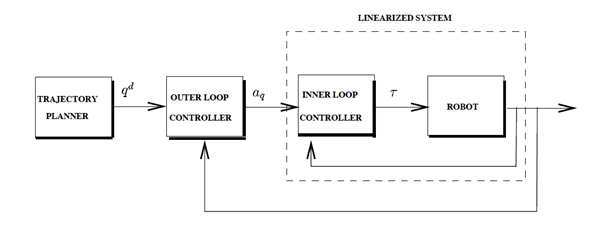
\includegraphics[width=.5\linewidth]{figs/Picture3}
		\caption{A  common 3 axis cartesian FDM 3D printer commonly consisting of 3 actuators}
		\label{figs/Picture3}
	\end{center}
\end{figure}

The computation of the nonlinear terms in Equation \ref{feedbacklin} is performed in the inner loop, perhaps with a dedicated microprocessor to obtain high computation speed. The computation of the additional term $a_q$ is performed in the outer loop. This separation of the inner loop and outer loop terms is important for several reasons. The structure of the inner loop control is fixed by Lagrange's equations. What control engineers traditionally think of as control system design is contained primarily in the outer loop. The outer loop control given in Equation \ref{PIDcont} is merely the simplest choice of outer loop control and achieves asymptotic tracking of joint space trajectories in the ideal case of perfect knowledge of the model given by Equation \ref{syseq}. However, one has complete freedom to modify the outer loop control to achieve various other goals without the need to modify the dedicated inner loop control. For example, additional compensation terms may be included in the outer loop to enhance the robustness to parametric uncertainty, unmodeled dynamics, and external disturbances. The outer loop control may also be modified to achieve other goals, such as tracking of task space trajectories instead of joint space trajectories, regulating both motion and force, etc. The inner loop/outer loop architecture thus unifies many robot control strategies from the literature. (Levine, 1996)

\subsection*{Shortfalls (further work here)}

No limits, often output saturation or fine tuning is required

\subsection{MPC}

\subsection*{Finite horizon optimal control}
LQR short term

\subsection*{Use of constraints}

We can tell the computer what it can and can’t do.  \\

MPC allows us to impose constraints on our system which are a result of physical constraints (actuator output and slew rate limits, displacement limits on the masses) and safety constraints (ensuring the net moment acting on the vertical beam is below a certain threshold). These are imposed as constrains on the states and the outputs of the system. (show math for this) 

\subsection*{Optimization}

Leveraging advances in SQP programs and theory 

\subsection*{NLMPC}

Nonlinear model predictive control (henceforth abbreviated as "NMPC"  is an optimization-based method for the feedback control of nonlinear systems. Its primary applications are stabilization and tracking problems, which we briefly introduce in order to describe the basic idea of model predictive control. (Grune and Pannek, 2017) \\

Suppose we are given a controlled process whose state $x(n)$ is measured at discrete time instants $t_n,n=0,1,2$, "Controlled" means that at each time instant we can select a control input $u(n)$ which 
influences the future behaviour of the state of the system. In tracking control, the task is to determine the control inputs $u(n)$ such that $x(n)$ follows a given reference $x^ref  (n)$ as good as possible. This means that if the current state is far away from the reference then we want to control the system towards the reference and if the current state is already close to the reference then we want to keep it there. In order to keep this introduction technically simple, we consider $x(n)\in X=R^d$ and $u(n)\in U=R^m$, furthermore we consider a reference which is constant and equal to $x_{*}=0$,i.e.,$x^ref (n)=x_{*}=0 $for all $n\geq 0$. With such a constant reference, the tracking problem reduces to a stabilization problem; in its full generality the tracking problem will be considered in Section \ref{tracking problem} (Grune and Pannek,2017) \\

Since we want to be able to react to the current deviation of $x(n)$from the reference value $x_{*}=0$, we would like to have $u(\eta)$ in feedback form, i.e, in the form $u(\eta)=\mu(x(n))$ for some map $\eta$ mapping the state $x \in X$ into the set $U$ of control values. The idea of model predictive control-linear or nonlinear-is now to utilize a model of the process in order to predict and optimize the future system behaviour. In this \textcolor{red}{book}, we will use models of the for.

\begin{equation}
	x^{\dotplus}=f(x,u)
\end{equation}

where $f: X \times U \rightarrow X$ is a known and in general nonlinear map which assigns to a state $x$ and a control
value $u$ the successor state $x^{+}$ at the next time instant. Starting
from the current state $x(n)$, for any given control sequence $u(0), \ldots, u(N-I)$ with horizon length
$N \geq 2$, we can now iterate (1.1) in order to construct a prediction trajectory $x_{u}$ defined by
$$
x_{u}(O)=x(n), \quad x_{u}(k+I)=f\left(x_{u}(k), u(k)\right), \quad k=0, \ldots, N-I
$$
Proceeding this way, we obtain predictions $x_{u}(k)$ for the state of the system $x(n+k)$ at time $t_{n+k}$ in
the future. Hence, we obtain a prediction of the behavior of the system on the discrete interval
$t_{n}, \ldots, t_{n+N}$ depending on the chosen control sequence $u(0), \ldots, u(N-1)$

Now we use optimal control in order to determine $u(0), \ldots, u(N-I)$ such that $x_{u}$ is as close as
possible to $x_{*}=0 .$ To this end, we measure the distance between $x_{u}(k)$ and $x_{*}=0$ for $k=0, \ldots, N-$ 1 by a function $1\left(\mathrm{x}_{\mathrm{u}}(\mathrm{k}), \mathrm{u}(\mathrm{k})\right)$. Here, we not only allow for penalizing the deviation of the state from
the reference but also if desired, the distance of the control values $u(k)$ to a reference control $u_{*}$, which
here we also choose as $u_{*}=0 .$ A common and popular choice for this purpose is the quadratic function
$$
\mathrm{l}\left(\mathrm{x}_{\mathrm{u}}(\mathrm{k}), \mathrm{u}(\mathrm{k})\right)=\left|\mathrm{x}_{\mathrm{u}}(\mathrm{k})\right|^{2}+\lambda|u(k)|^{2}
$$
where ||. || denotes the usual Euclidean norm and $\lambda \geq 0$ is a weighting parameter for the control, which
could also be chosen as 0 if no control penalization is desired.
The optimal control problem now reads
$$
\mathrm{J}(\mathrm{x}(\mathrm{n}), \mathrm{u}(\cdot)):=\sum_{\mathrm{k}=0}^{\mathrm{N}-1} \mathrm{l}\left(\mathrm{x}_{\mathrm{u}}(\mathrm{k}), \mathrm{u}(\mathrm{k})\right)
$$
with respect to all admissible $\ \quad I$ control sequences $\mathrm{u}(0), \ldots, \mathrm{u}(\mathrm{N}-1)$ with $x_{u}$ generated by (1.2)
Let us assume that this optimal control problem has a solution which is given by the minimizing control
sequence $u^{*}(0), \ldots, u^{*}(N-I),$ i.e.
$$
\min _{u(0), \ldots, u(N-1)} J(x(n), u(\cdot))=\sum_{k=0}^{N-1} l\left(x_{u^{*}}(k), u^{*}(k)\right)
$$
In order to get the desired feedback value $\mu(x(n)),$ we now $\operatorname{set} \mu(x(n)):=u^{*}(0),$
i.e., we apply the first element of the optimal control sequence. This procedure is sketched in Fig. 1.1 .


At the following time instants $t_{n+1}, t_{n+2}$, we repeat the procedure with the new measurements
$x(n+1), x(n+2),$ in order to derive the feedback values $\mu(x(n+1)), \mu(x(n+2)),$ In other words,
we obtain the feedback law $\mu$ by an iterative online optimization over the predictions generated by our
model $(1.1) .^{2}$ This is the first key feature of model predictive control. (Grüne and Pannels, 2017 )

\begin{figure}[H]
	\begin{center}
		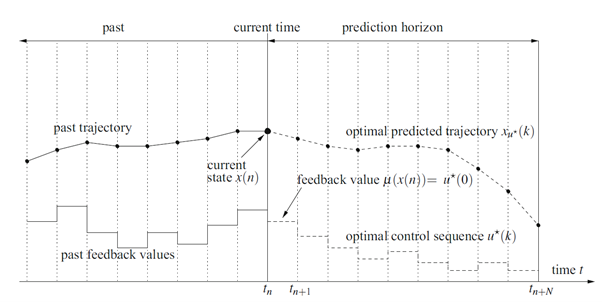
\includegraphics[width=.5\linewidth]{figs/Picture7}
		\caption{A  common 3 axis cartesian FDM 3D printer commonly consisting of 3 actuators}
		\label{figs/Picture7}
	\end{center}
\end{figure}

Fig. 4 Mustration of the NMPC step at time $t_{n}$

From the prediction horizon point of view, proceeding this iterative way the trajectories $x_{u}(k), k=$
$0, \ldots, N$ provide a prediction on the discrete interval $t_{n}, \ldots, t_{n+N}$ at time $t_{n},$ on the interval
$t_{n+1}, \ldots, t_{n+N+1}$ at time $t_{n+l},$ on the interval $t_{n+2}, \ldots, t_{n+N+2}$ at time $t_{n+3}$ and so on. Hence, the
prediction horizon is moving and this moving horizon is the second key feature of model predictive
control. (Grüne and Pannek, 2017 )

Regarding terminology, another term which is often used alternatively to model predictive control is
receding horizon control. While the former expression stresses the use of model-based predictions, the
latter emphasizes the moving horizon idea. Despite these slightly different literal meanings, we prefer
and follow the common practice to use these names synonymously. The additional term nonlinear
indicates that our model (1.1) need not be a linear map. (Grüne and Rannels 2017 )
(Use of nonlinear constraints)
(No need for linearization
Can use complex ode solvers like ode45 to accurately represent systen


%%%%%%%%%%%%%%%%%%%%%%%%%%%%%%%%%%%%%%%%%%%
\newpage
\section*{Chapter 2}
\addcontentsline{toc}{section}{Chapter 2}
\section{System Overview}
In your own words, step by step, what does the program do to simulate the system

\subsection{Flow diagram}

\begin{figure}[H]
	\begin{center}
		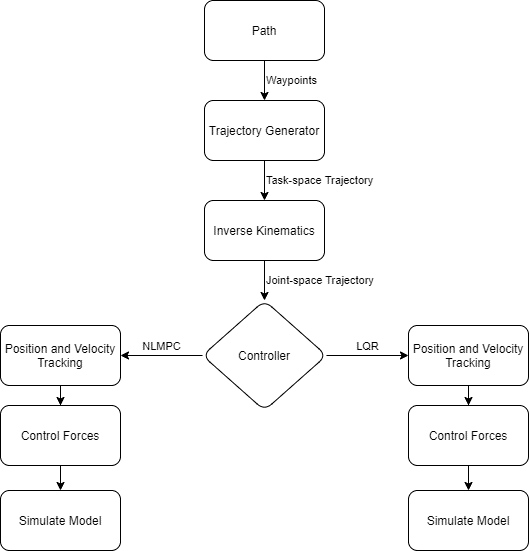
\includegraphics[width=.5\linewidth]{figs/Picture4}
		\caption{A  common 3 axis cartesian FDM 3D printer commonly consisting of 3 actuators}
		\label{figs/Picture4}
	\end{center}
\end{figure}

\section{Crane System Modelling}

\subsection{Tower Crane System}
The tower crane model is based on \ref{figs/Picture4} with key properties shown in table \ref{tab:physical param}. This design

\begin{figure}[H]
	\begin{center}
		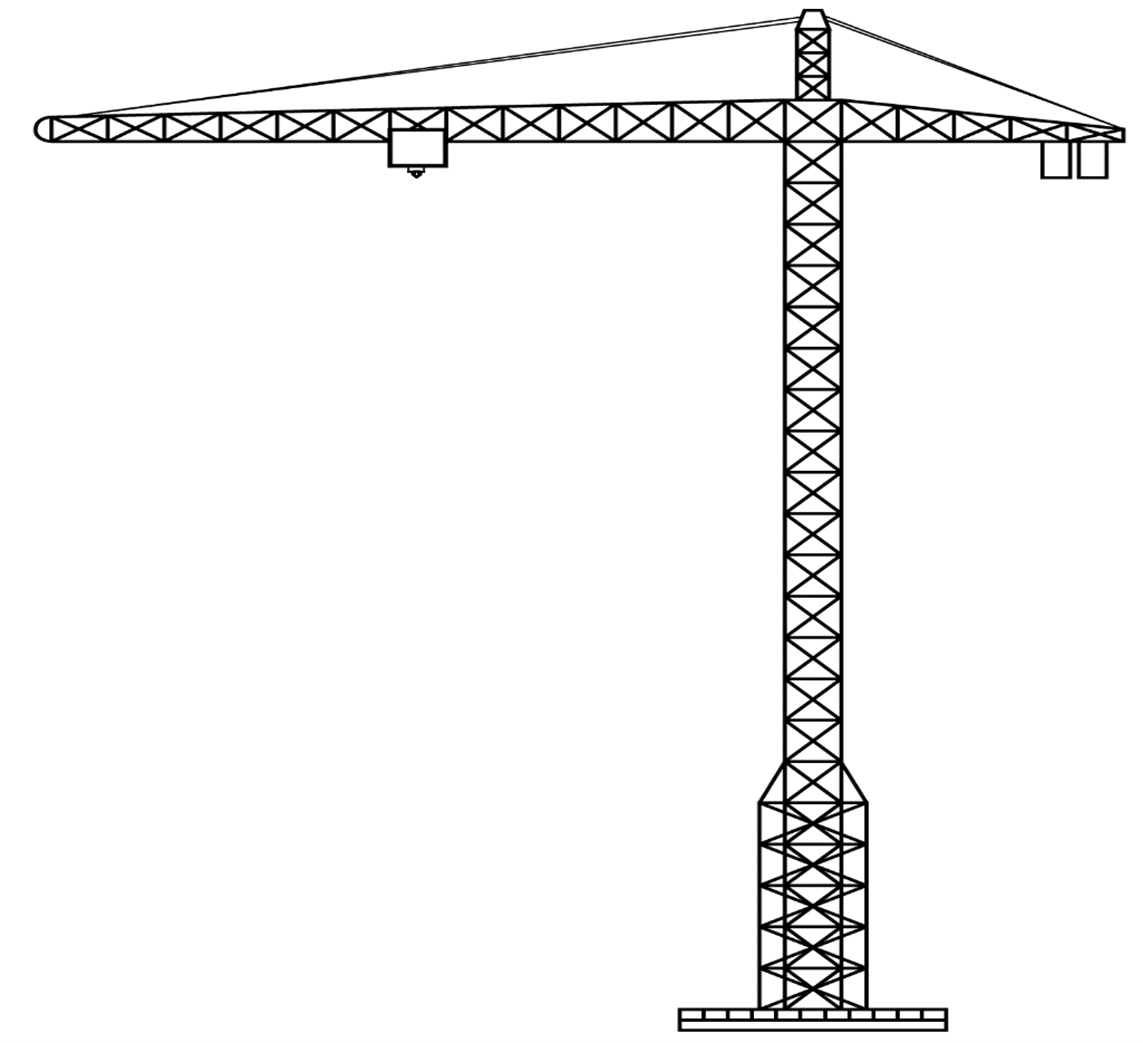
\includegraphics[width=.5\linewidth]{figs/Picture5}
		\caption{A  common 3 axis cartesian FDM 3D printer commonly consisting of 3 actuators}
		\label{figs/Picture5}
	\end{center}
\end{figure}

\subsection*{Assumptions}
\begin{itemize}
	\item There will be 4 actuators controlling the crane. Actuator 1 and 2 will slide the end effector and counterweight along their respective gantry. Actuator 3 will rotate the crane about the tower and actuator 4 will slide the crane up and down the tower. 
	\item Instead of a hook, the end effector will be a nozzle which deposits filament which is stored externally from the crane and pumped through piping.
	
\end{itemize}


\begin{table}[H] \centering 
	\caption{Table meh}
	\begin{tabular}{ll}
		\hline
		Parameters              & Values \\ \hline 
		End Effector (m\_1)     & 1 kg   \\ 
		Counterweight (m\_2)    & 3.6 kg \\ 
		Horizontal Beam length  & 1.4 m  \\ 
		Vertical Beam length    & 1 m    \\ 
		Mass of Horizontal beam & 1.4 kg \\ 
		Mass of Vertical Beam   & 5 kg  
	\end{tabular}
	\label{tab:physical param}
\end{table}

The table \ref{tab:physical param} above represents the values of the constable assumed in the modelling and simulation of the project.


\subsection{Fully Actuated System}

In the study of mechanisms are acquired two concepts very important such as the direct and indirect action. The first consists of movement of elements by action of an actuator, while the second consists of the action of motion transmitted by another interconnected element. Such movements are known as DOF, so that mechanical systems or mechanisms can be classified depending on the number of DOF and the number of actuators. The fully actuated mechanical systems are those having the same number of DOF and actuators. \\

Underactuated mechanical systems are those with fewer actuators than DOF. It is important to highlight the advantages of underactuated systems, since if they do not have advantages over fully actuated mechanical systems, it will not make sense its development. The main advantages present in underactuated systems are energy saving and control efforts. However, these systems are intended to perform the same functions of fully actuated systems without their disadvantages. (Duarte Madrid et al., 2017)


\subsection{Mathematical Model}

The tower crane is converted into a kinematic model and states are assigned: 
\begin{equation}
q = 
\begin{bmatrix}
r1 \\ r2 \\ \theta \\ z
\end{bmatrix}
\end{equation}

Which can be used to describe the motion of mass 1, mass 2, beam 1 and beam 2

\begin{figure}[H]
	\begin{center}
		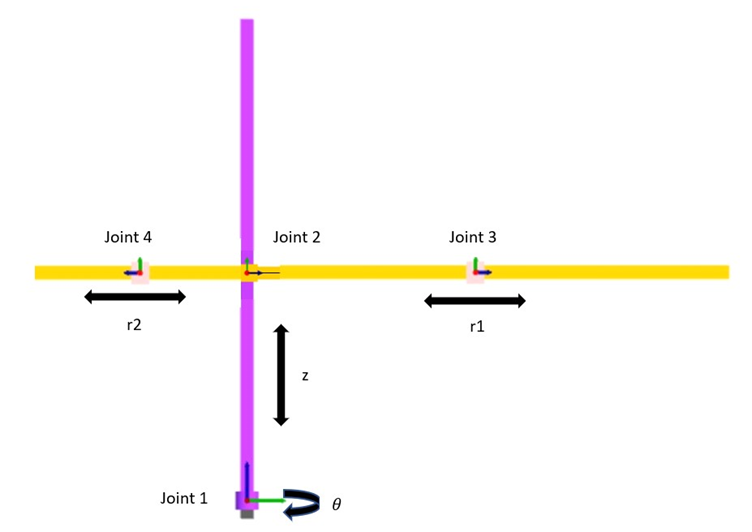
\includegraphics[width=.5\linewidth]{figs/Picture6}
		\caption{A  common 3 axis cartesian FDM 3D printer commonly consisting of 3 actuators}
		\label{figs/Picture6}
	\end{center}
\end{figure}

\subsection{Forward Kinematics of the crane system}

As it can be seen in the figure above joint 3 and joint 4 are not in a continuous kinematic chain therefore separate transformations were needed.  The table below shows all the parameters that were required to obtain the forward kinematics for joint three and joint 4.

\begin{table}[] \centering 
	\caption{DH Parameters table for base to joint 3 and joint 4}
	\begin{tabular}{llllll}
		\hline
		Joint \# & Joint Type & Joint offset 'd' & Link length 'a' & Joint angle ‘$\theta$’ & Twist angle'$\alpha$' \\ \hline
		1        & Revolute   & 0                & 0               & 0               & 0              \\
		2        & Prismatic  & z                & 0               & 0              & -90            \\
		3        & Prismatic  & r2               & 0               & 0               & 0             
	\end{tabular} \vspace{5mm}

	\begin{tabular}{llllll}
	\hline
	Joint \# & Joint Type & Joint offset 'd' & Link length 'a' & Joint angle ‘$\theta$’ & Twist angle'$\alpha$' \\ \hline
	1        & Revolute   & 0                & 0               & 0               & 0              \\
	2        & Prismatic  & z                & 0               & 0              & 90            \\
	4        & Prismatic  & r1               & 0               & 0               & 0             
\end{tabular}

\end{table}


Using the * DH equation mentioned in the background with the identified parameters in Table 1 a homogenous transformation matrix $A_{n}^(n-1)$ is produced representing transformation from $n-1$ to $n$. 

\begin{equation}
	T_n^0 (q)=A_1^0 (q_1 ) A_2^1 (q_2 ) \dots A_{n}^{n-1} (q_n )
\end{equation}

The general equation for transformation between continuous kinematic chain is represented above.

\begin{equation}
	T_3^0 (q)=A_1^0 (q_1 ) A_2m1^1 (q_2 ) A_3m1^2m1 (q_3 )
\end{equation}
\begin{equation}
T_4^0 (q)=A_1^0 (q_1 ) A_2m2^1 (q_2 ) A_4m2^2m2 (q_4 )
\end{equation}

Since we do not have a continuous kinematic chain, we will require two transformation equations as represented above. $T_3^0$ is for the transformation from origin to $r_2$ while $T_4^0$ is the transformation from origin to $r_1$, where $r_1$ is considered to be the position of the end effector for this project. \\
These transformations are beneficial as they are used in the project for converting joint space coordinates to cartesian coordinates which is also used simulation, verification and visualisation purposes.

Post the final A matricies (aka, the numbers inside them at a random position to demonstrate, then post a photo of the crane with the same numbers in each spot.  \\
FKM([.5,(-0.08+.5+0.5)/3.6,pi/2,.5])

\begin{align*}
	A_0^1 &= 
	\begin{bmatrix}
	0 & -1 & 0 & 0 \\
	1 & 0 & 0 & 0\\
	0 & 0 & 1 & 0\\
	0 & 0 & 0 & 1\\
	\end{bmatrix} & 		
	A_{2m2}^1 &= 
	\begin{bmatrix}
	-1 & 0 & 0 & 0 \\
	0 & 1 & -1 & 0\\
	0 & -1 & 0 & 0.5\\
	0 & 0 & 0 & 1\\
	\end{bmatrix} &	
		A_0^1 &= 
	\begin{bmatrix}
	0 & 0 & 1 & 0 \\
	1 & 0 & 0 & 0\\
	0 & -1 & 1 & 0\\
	0 & 0 & 0 & 1\\
	\end{bmatrix} \\ \vspace{5mm}
		A_0^1 &= 
	\begin{bmatrix}
	1 & 0 & 0 & 0 \\
	0 & 0 & 1 & 0\\
	0 & -1 & 0 & 0.5\\
	0 & 0 & 0 & 1\\
	\end{bmatrix} & 		
	A_{2m2}^1 &= 
	\begin{bmatrix}
	1 & 0 & 0 & 0 \\
	0 & 1 & 0 & 0\\
	0 & 0 & 1 & 0.2556\\
	0 & 0 & 0 & 1\\
	\end{bmatrix} &	
	A_0^1 &= 
	\begin{bmatrix}
	0 & 0 & 1 & 0.5 \\
	1 & 0 & 0 & 0\\
	0 & -1 & 0 & 0.5\\
	0 & 0 & 0 & 1\\
	\end{bmatrix} \\ \vspace{5mm}
			A_0^1 &= 
	\begin{bmatrix}
	1 & 0 & 0 & 0 \\
	0 & 1 & 0 & 0\\
	0 & 0 & 1 & 0.5\\
	0 & 0 & 0 & 1\\
	\end{bmatrix} & 		
	A_{2m2}^1 &= 
	\begin{bmatrix}
	1 & -1 & 0 & 0 \\
	1 & 0 & 0 & 0\\
	0 & 0 & 1 & 0.2556\\
	0 & 0 & 0 & 1\\
	\end{bmatrix} &	
	A_0^1 &= 
	\begin{bmatrix}
	0 & 0 & 1 & 0.5 \\
	1 & 0 & 0 & 0\\
	0 & -1 & 0 & 0.5\\
	0 & 0 & 0 & 1\\
	\end{bmatrix} \\
\end{align*}

\begin{figure}[H]
	\begin{center}
		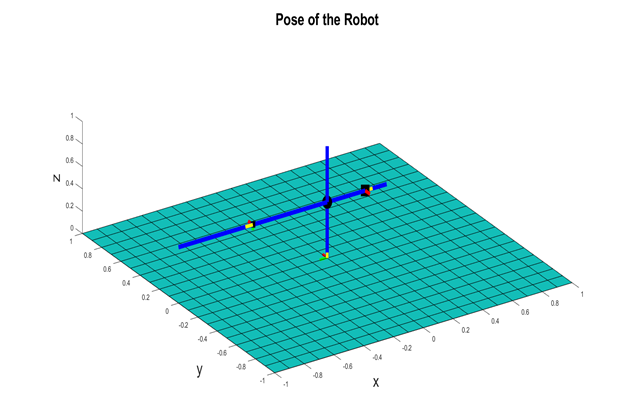
\includegraphics[width=.5\linewidth]{figs/Picture8}
		\caption{A  common 3 axis cartesian FDM 3D printer commonly consisting of 3 actuators}
		\label{figs/Picture8}
	\end{center}
\end{figure}

\subsection{Inverse kinematics of crane system}

Using simple cartesian to polar coordinate transformation following equations are obtained as listed
below this also includes calculation for position of $r_{2}$ making $\sum$ Moments $=0$

\begin{align}
	 r_{1} & =\sqrt{x^{2}+y^{2}} \\ 
	\theta & =\arctan \left|\frac{y}{x}\right| \\
	r_{2} &=\frac{b e a m \operatorname{torque}+m_{1} * r_{1}}{m_{2}} \\ 
	z & =z 
\end{align}


\section{Modelling a crane system using Lagrangian}

In order to calculate the Lagrangian of a system, we compute all the potential energies which are then
subtracted from the kinetic energies of the system.
$$
\begin{array}{c}
\mathcal{L}=T-V \\
\mathcal{L}(\boldsymbol{q}(\boldsymbol{t}), \dot{\boldsymbol{q}}(\boldsymbol{t}))=T(\boldsymbol{q}(\boldsymbol{t}), \dot{\boldsymbol{q}}(\boldsymbol{t}))-\boldsymbol{V}(\boldsymbol{q}(\boldsymbol{t})) \\
\mathcal{L}=\frac{\mathbf{1}}{2}\left(\boldsymbol{m}_{1} \boldsymbol{r}_{1}+\boldsymbol{m}_{2} \dot{\boldsymbol{r}}_{2}^{2}+\left(\boldsymbol{m}_{1}+\boldsymbol{m}_{2}+\boldsymbol{m}_{b}\right) \dot{z}^{2}+\boldsymbol{m}_{1} \boldsymbol{r}_{1}^{2} \dot{\boldsymbol{\theta}}^{2}+\boldsymbol{m}_{2} \boldsymbol{r}_{2}^{2} \dot{\boldsymbol{\theta}}^{2}+\boldsymbol{I}_{b} \dot{\boldsymbol{\theta}}^{2}\right)-g \mathbf{z}\left(\boldsymbol{m}_{1}+\boldsymbol{m}_{2}\right. \\
\left.+\boldsymbol{m}_{\boldsymbol{b}}\right)
\end{array}
$$
Where $m_{1}$ is mass of joint $3, m_{2}$ is mass of joint $4, m_{b}$ is mass of the horizontal beam and
$$
I_{b}=\left(\frac{1}{12} m l_{c m}^{2}+m d^{2}\right)+\left(\frac{1}{2} m r^{2}\right), \text { using paralled axis theorem }
$$
Listed above are all the kinetic and potential energies taken into account which are linear motion of $m$
along the beam (nozzle), linear motion of $m_{2}$ along the beam, linear motion of all masses along $z$ axis,
angular motion of $m_{l}$, angular motion of $m_{2}$, angular motion of beam and potential energy due to
gravity of all the masses respectively.
We now calculate Euler-Lagrange equations using the following:
$$
\begin{array}{c}
\frac{d}{d t}\left(\frac{\partial \mathcal{L}(q, \dot{q})}{\partial \dot{q}_{i}}\right)-\frac{\partial \mathcal{L}(q, \dot{q})}{\partial q_{i}}=\tau_{i} \\
\frac{m_{1} \dot{r}_{1}}{m_{2} \dot{r}_{2}} \\
\frac{d}{d t}\left[\begin{array}{c}
m_{1} r_{1} \dot{\theta}^{2} \\
m_{2} r_{2} \theta^{2} \\
0 \\
-\left(m_{1}+m_{2}+m_{b}\right) g
\end{array}\right]=\left[\begin{array}{c}
F_{1} \\
F_{2} \\
\tau \\
F_{z}
\end{array}\right] \\
\left.\left(m_{1}+m_{2}+m_{b}\right) \dot{z}^{2} \dot{\theta}+m_{2} r_{1}^{2} \dot{\theta}+I_{b} \dot{\theta}\right]-\left[\begin{array}{c}
F_{1} \\
F_{2} \\
\tau \\
F_{z}
\end{array}\right]
\end{array}
$$
Second order equations listed below
$$
\ddot{\mathrm{r}}_{1}=\frac{\mathrm{F}_{1}+\mathrm{m}_{1} \mathrm{r}_{1} \dot{\theta}^{2}}{\mathrm{~m}_{1}}
$$

$$
\begin{array}{c}
\ddot{\mathrm{r}}_{2}=\frac{\mathrm{F}_{2}+\mathrm{m}_{2} \mathrm{r}_{2} \dot{\theta}^{2}}{\mathrm{~m}_{2}} \\
\ddot{\theta}=\frac{\tau-2\left(\mathrm{~m}_{1} \mathrm{r}_{1} \dot{\mathrm{r}}_{1}+\mathrm{m}_{2} \mathrm{r}_{2} \dot{\mathrm{r}}_{2}\right) \dot{\theta}}{\mathrm{m}_{1} \mathrm{r}_{1}^{2}+\mathrm{m}_{2} \mathrm{r}_{2}^{2}+\mathrm{I}_{\mathrm{b}}} \\
\ddot{\mathrm{z}}=\frac{\mathrm{F}_{\mathrm{z}}-\left(\mathrm{m}_{1}+\mathrm{m}_{2}+\mathrm{m}_{\mathrm{b}}\right) \mathrm{g}}{\left(\mathrm{m}_{1}+\mathrm{m}_{2}+\mathrm{m}_{\mathrm{b}}\right)}
\end{array}
$$
Dynamic equation of an n-link robot in the matrix form is listed below
$$
M(q) \ddot{q}+C(q, \dot{q}) \dot{q}+g(q)=u
$$
Where
$$
M(\boldsymbol{q}) \ddot{q}=\left[\begin{array}{cccc}
m_{1} & 0 & 0 & 0 \\
0 & m_{2} & 0 & 0 \\
0 & 0 & m_{1} r_{1}^{2}+m_{2} r_{2}^{2}+I_{b} & 0 \\
0 & 0 & 0 & m_{1}+m_{2}+m_{b}
\end{array}\right]\left[\begin{array}{c}
\ddot{r}_{1} \\
\ddot{r}_{2} \\
\ddot{\theta} \\
\ddot{z}
\end{array}\right]
$$
$C(q, \dot{q}) \dot{q}=\left[\begin{array}{cccc}0 & 0 & -m_{1} r_{1} \dot{\theta} & 0 \\ 0 & 0 & -m_{2} r_{2} \theta & 0 \\ 2 m_{1} r_{1} \dot{\theta} & 2 m_{2} r_{2} \dot{\theta} & 0 & 0 \\ 0 & 0 & 0 & 0\end{array}\right]\left[\begin{array}{c}r_{1} \\ r_{2} \\ \theta \\ \dot{z}\end{array}\right], \quad g(q)=\left[\begin{array}{c}0 \\ 0 \\ 0 \\ g\left(m_{1}+m_{2}+m_{b}\right)\end{array}\right]$
$u=\left[\begin{array}{c}F_{1} \\ F_{2} \\ \tau \\ F_{z}\end{array}\right]$

\section{Simulating in MATLAB}
Setting up a run script\\
What timestep did you use? Why? \\
ODE45 returns a massive vector of times and values, how did you take the last value out?\\


Animating a script\\
Post a snippit of the code you used to animate it, \\
How does plot3 work? Do you play it frame by frame?\\


%%%%%%%%%%%%%%%%%%%%%%%%%%%%%%%%%%%%%%%%%%%
\newpage
\section*{Chapter 3}
\addcontentsline{toc}{section}{Chapter 3}
\section{Motion control and Trajectory Generation}

Given a set of wav-points that describes the build order of a set of walls, we need a reference to track
that is achievable by the machinery. This is a non-trivial problem for a few reasons.
\subsection{Trapezoidal Model of Speed}
In $3 \mathrm{D}$ extrusion printing, there is an optimum speed at which the printer head can lay down the ideal
thickness of material. On any run of continuous printing, it is preferred that the head starts from rest but
accelerates at a reasonable rate to this optimum speed which is maintained until near the end of the run
when deceleration returns the head to rest. In the simplest case of a run along a straight-line segment,
the acceleration and deceleration will be constant and of the same size giving a trapezoidal speed profile.
This trapezoidal profile is illustrated in Fig. $5 .$

\begin{figure}[H]
\begin{center}
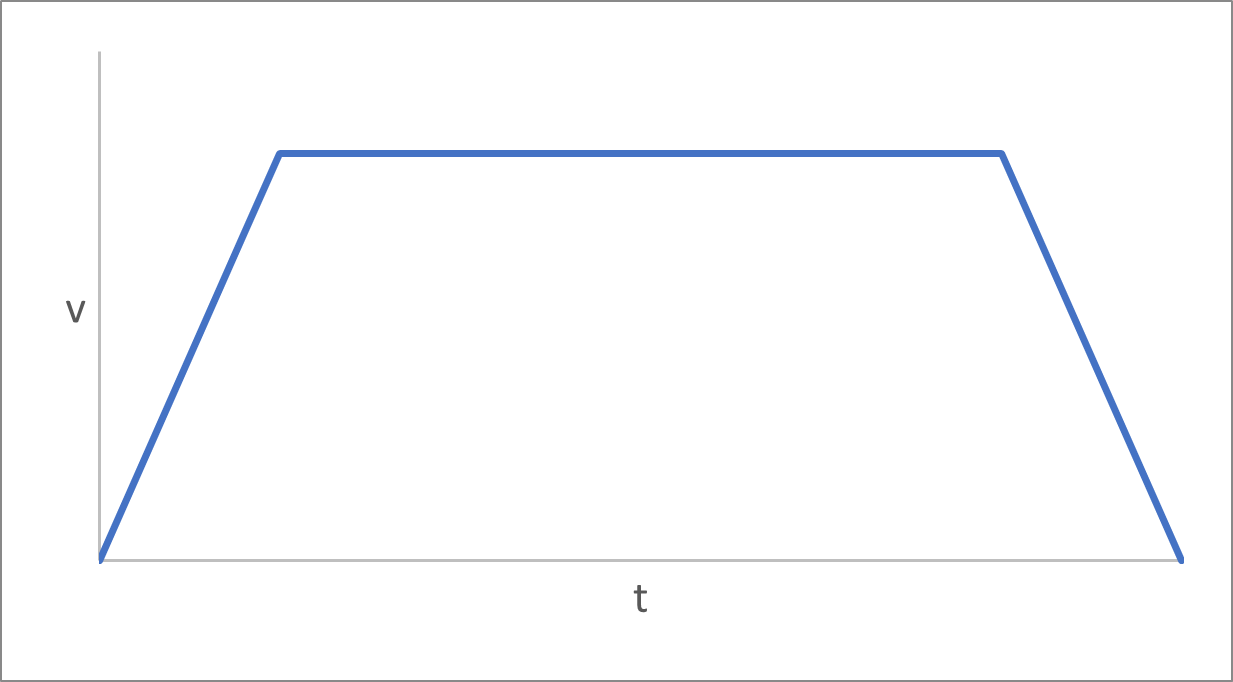
\includegraphics[width=.5\linewidth]{figs/Picture9}
\caption{A  common 3 axis cartesian FDM 3D printer commonly consisting of 3 actuators}
\label{figs/Picture9}
\end{center}
\end{figure}

Fig. 7 Trapezoidal profile of speed (v) against time (t
With time variable $t,$ distance travelled $s,$ velocity $v=\frac{d s}{d t} \mathrm{~m} / \mathrm{s},$ preferred acceleration rate $a,$ optimum
head speed $u$ and total distance to travel $d$, the requirements are that:
\begin{itemize}
\item The run starts at rest at time $t=0$ with no distance travelled so $s(0)=t(0)=0$
\item The head accelerates with constant acceleration $a$ until time $t_{1}$ when speed is $u$ so $v\left(t_{1}\right)=u$
\item The velocity is held constant until time $t$
\item The head decelerates at a constant rate until it comes to rest at time $t_{e}$ so $v\left(t_{\theta}\right)=0$
\item The total distance travelled is $d$ so $s\left(t_{e}\right)=a$
\end{itemize}

Then the dynamic system is specified by:
$$
\frac{d v}{d t}=\left\{\begin{array}{ll}
a & 0 \leq t \leq t_{1} \\
0 & t_{1}<t \leq t_{2} \\
-a & t_{2}<t \leq t_{e}
\end{array}\right.
$$


Assuming that, with the constant acceleration, the distance to be travelled is long enough to allow the
optimum speed to be reached, the speed and distance travelled are then given by:
$$
\begin{array}{c}
v=\left\{\begin{array}{cc}
\text { at } & 0 \leq \mathrm{t} \leq \mathrm{t}_{1} \\
\mathrm{u} & \mathrm{t}_{1}<\mathrm{t} \leq \mathrm{t}_{2} \\
\mathrm{u}-\mathrm{a}\left(\mathrm{t}-\mathrm{t}_{2}\right) & \mathrm{t}_{2}<\mathrm{t} \leq \mathrm{t}_{\mathrm{e}}
\end{array}\right. \\
s=\left\{\begin{array}{cc}
\mathrm{at}^{2} / 2 & 0 \leq \mathrm{t} \leq \mathrm{t}_{1} \\
\mathrm{u}\left(\mathrm{t}-\mathrm{t}_{1}\right)+\frac{\mathrm{u}^{2}}{2 \mathrm{a}} & \mathrm{t}_{1}<\mathrm{t} \leq \mathrm{t}_{2} \\
\mathrm{u}\left(\mathrm{t}-\mathrm{t}_{1}\right)-\mathrm{a}\left(\mathrm{t}-\mathrm{t}_{2}\right)^{2} / 2+\frac{\mathrm{u}^{2}}{2 \mathrm{a}} & \mathrm{t}_{2}<\mathrm{t} \leq \mathrm{t}_{\mathrm{e}}
\end{array}\right.
\end{array}
$$
With $v\left(\mathrm{t}_{1}\right)=a \mathrm{t}_{1}=u, \mathrm{t}_{1}=u / a .$ To ensure the optimum speed can be reached, the distance travelled
at the end of acceleration must be less than half the total distance. That is
$$
s\left(t_{1}\right)=\frac{a t_{1}^{2}}{2}=\frac{u^{2}}{2 a}<\frac{d}{2}
$$
Therefore, this condition can be expressed as $\mathrm{d}>\frac{\mathrm{u}^{2}}{\mathrm{a}} .$ By symmetry, $\mathrm{t}_{\mathrm{e}}-\mathrm{t}_{2}=\mathrm{t}_{1}=\frac{\mathrm{u}}{\mathrm{a}}$ so
$$
s\left(t_{e}\right)=u t_{e}-\frac{u^{2}}{a}-\frac{a\left(\frac{u}{a}\right)^{2}}{2}+\frac{u^{2}}{2 a}=u t_{e}-\frac{u^{2}}{a}=d
$$
to give $t_{e}=\frac{d}{u}+\frac{u}{a}$ and $t_{2}=\frac{d}{u}$
In practice, any continuous extrusion run will, at best, consist of a sequence of straight-line segments
of reasonable length allowing optimum speed to be reached on each segment. However, there is an
issue of balancing the desire for constant speed against maintaining rigid adherence to the linear
sections. The generation of curves requires approximation by many very small line segments where the
above model is not at all suitable. To deal with the most general cases, more refined approaches are
needed which includes smooth motion that uses the final velocity and acceleration as the initial values
for the following segment thus maintaining the velocity.

\subsection{Multi-segment Multi-Axis Trajectory}
Multi-segment multi-axis trajectory is a way of generating a trajectory based on via points. In the use of robotics there is usually a requirement to move smoothly along a path through one or more via points without stopping. It is a requirement for this project to have a continuous trajectory that involves not stopping at the points this is due to the continuous extrusion from the nozzle of the printer. It could cause an inconsistency on the texture of the extrusion. \\
To make the extrusion more uniform the velocity has to be constrained to suit the robot’s actuators slew rates and the maximum extrusion limit. The path then compromises of linear segments with fifth order quintic polynomials. The trajectory is generated by using the via points with velocity and acceleration limits and a position and a time is recorded for each time segment to suit the frequency of the controller action.

\begin{figure}[H]
	\begin{center}
		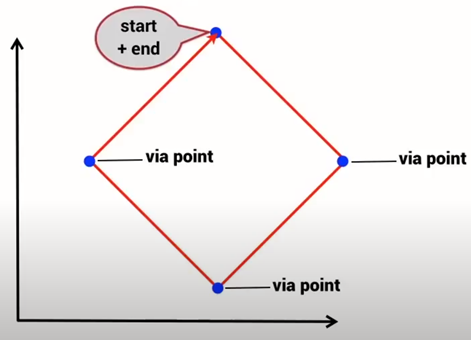
\includegraphics[width=.5\linewidth]{figs/Picture10}
		\caption{A  common 3 axis cartesian FDM 3D printer commonly consisting of 3 actuators}
		\label{figs/Picture10}
	\end{center}
\end{figure}


The 5 th order quintic polynomial is used as it has six coefficients that allows it to meet its six boundary
conditions which are initial and final positions, velocities and accelerations. These polynomials are
given by the following equations below.
$$
\begin{array}{c}
q(t)=a_{0}+a_{1} t+a_{2} t^{2}+a_{3} t^{3}+a_{4} t^{4}+a_{5} t^{5} \\
q_{0}=a_{0}+a_{1} t_{0}+a_{2} t_{0}^{2}+a_{3} t_{0}^{3}+a_{4} t_{0}^{4}+a_{5} t_{0}^{5} \\
v_{0}=a_{1}+2 a_{2} t_{0}+3 a_{3} t_{0}^{2}+4 a_{4} t_{0}^{3}+5 a_{5} t_{0}^{4} \\
\alpha_{0}=2 a_{2}+6 a_{3} t_{0}+12 a_{4} t_{0}^{2}+20 a_{5} t_{0}^{3} \\
q_{f}=a_{0}+a_{1} t_{f}+a_{2} t_{f}^{2}+a_{3} t_{f}^{3}+a_{4} t_{f}^{4}+a_{5} t_{f}^{5} \\
v_{f}=a_{1}+2 a_{2} t_{f}+3 a_{3} t_{f}^{2}+4 a_{4} t_{f}^{3}+5 a_{5} t_{f}^{4} \\
\alpha_{f}=2 a_{2}+6 a_{3} t_{f}+12 a_{4} t_{f}^{2}+20 a_{5} t_{f}^{3} \\
q_{0}=\text { initial position } \\
v_{0}=\text { initial velocity } \\
\alpha_{0}=\text { initial acceleration }
\end{array}
$$
where,
$$
\begin{array}{l}
q_{f}=\text { final position } \\
v_{f}=\text { final velocity } \\
\alpha_{f}=\text { final acceleration }
\end{array}
$$
\subsection{Blend feature} 
The trajectory starts from $q_{1}$ at rest and finishes at a point $q_{M}$ and comes to a stop. However, for all the
point in between $q_{1}$ and $q_{M}$ its moves through or closer to the intermediate configurations in a
continuous motion. The over constraints the problem and in order to achieve the intermediate
configuration with continuous motion, the ability to reach each intermediate configuration exactly, is
surrendered. To make it easier to understand a one-dimensional case is shown in Fig. 7

The robot starts from $\mathrm{q}_{1}$ at rest and finishes at $\mathrm{q}_{\mathrm{M}}$ at rest, but moves through (or close to) the
intermediate configurations without stopping. The problem is over constrained and in order to attain
continuous velocity we surrender the ability to reach each intermediate configuration. This is easiest to
understand for the 1 -dimensional case shown in Fig. $3.5 .$ The motion comprises linear motion segments
with polynomial blends, but here we choose quintic polynomials because they are able to match
boundary conditions on position, velocity and acceleration at their start and end points.

\begin{figure}[H]
	\begin{center}
		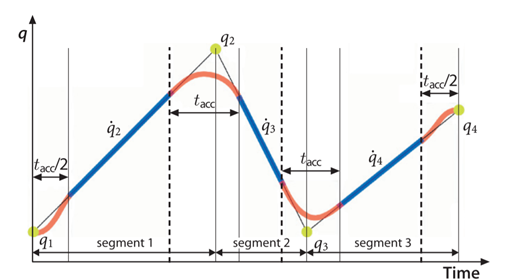
\includegraphics[width=.5\linewidth]{figs/Picture11}
		\caption{A  common 3 axis cartesian FDM 3D printer commonly consisting of 3 actuators}
		\label{figs/Picture11}
	\end{center}
\end{figure}

The first segment of the trajectory accelerates from the initial configuration $q_{1}$ and zero velocity, and
joins the line heading toward the second configuration $q_{2}$. The blend time is set to be a constant $t_{\mathrm{acc}}$
and $t_{\text {acc }} / 2$ before reaching $q_{2}$ the trajectory executes a polynomial blend, of duration $t_{\text {acc }},$ onto the line
from $q_{2}$ to $q_{3},$ and the process repeats. The constant velocity $q_{k}$ can be specified for each segment. The
average acceleration during the blend is
$$
\ddot{q}=\frac{\dot{q}_{k+1}-\dot{q}_{k}}{t_{a c c}}
$$

\section{Linear Quadratic Regulator (LQR) Control}

The LQR requires a linear model to be converted into a state-space model mentioned below
$$
\begin{array}{l}
\dot{x}=A x+B u \\
y=C x+D u
\end{array}
$$
In the modelling section we have calculated 4 Euler Lagrange egyations's of motion. These are second
order nonlinear equations. For us to be able to control the system with LQR we need to convert the
equations into first order and then use a technique called feedback linearisation to linearize the model.
Second order differential equations:
$$
\begin{array}{c}
\ddot{\mathrm{r}}_{1}=\frac{\mathrm{F}_{1}+\mathrm{m}_{1} \mathrm{r}_{1} \dot{\theta}^{2}}{\mathrm{~m}_{1}} \\
\ddot{r}_{2}=\frac{\boldsymbol{F}_{2}+\boldsymbol{m}_{2} \boldsymbol{r}_{2} \dot{\theta}^{2}}{\boldsymbol{m}_{2}} \\
\ddot{\boldsymbol{\theta}}=\frac{\boldsymbol{\tau}-2\left(\boldsymbol{m}_{1} \boldsymbol{r}_{1} \dot{\boldsymbol{r}}_{1}+\boldsymbol{m}_{2} \boldsymbol{r}_{2} \dot{\boldsymbol{r}}_{2}\right) \dot{\boldsymbol{\theta}}}{\boldsymbol{m}_{1} \boldsymbol{r}_{1}^{2}+\boldsymbol{m}_{2} \boldsymbol{r}_{2}^{2}+\boldsymbol{I}_{b}} \\
\ddot{\mathbf{z}}=\frac{\boldsymbol{F}_{z}-\left(\boldsymbol{m}_{1}+\boldsymbol{m}_{2}+\boldsymbol{m}_{b}\right) g}{\left(\boldsymbol{m}_{1}+\boldsymbol{m}_{2}+\boldsymbol{m}_{b}\right)}
\end{array}
$$
For ease of calculation and simplification we have kept the first 4 states as joint positions and the next
four states as joint velocities.
$$
x=\left[\begin{array}{l}
x_{1} \\
x_{2} \\
x_{3} \\
x_{4} \\
x_{5} \\
x_{6} \\
x_{7} \\
x_{8}
\end{array}\right]=\left[\begin{array}{c}
r_{1} \\
r_{2} \\
\theta \\
z \\
\dot{r}_{1} \\
\dot{r}_{2} \\
\dot{\theta} \\
\dot{z}
\end{array}\right]
$$

The model below is not represented by first order differential equations
$$
\left[\begin{array}{c}
\mathrm{x}_{5} \\
\mathrm{x}_{6} \\
\mathrm{x}_{7} \\
\mathrm{x}_{8} \\
\dot{\mathrm{x}}_{1} \\
\dot{\mathrm{x}}_{2} \\
\dot{\mathrm{x}}_{3} \\
\dot{\mathrm{x}}_{4} \\
\dot{\mathrm{x}}_{5} \\
\dot{\mathrm{x}}_{6} \\
\dot{\mathrm{x}}_{7} \\
\dot{\mathrm{x}}_{8}
\end{array}\right]=\left[\begin{array}{c}
{\mathrm{r}}_{1} \\
\dot{\mathrm{r}}_{2} \\
\dot{\theta} \\
\dot{\mathrm{z}} \\
\ddot{\mathrm{r}}_{1} \\
\ddot{\mathrm{r}}_{2} \\
\ddot{\theta} \\
\ddot{z}
\end{array}\right]=\left[\begin{array}{c}
\frac{\mathrm{F}_{1}+\mathrm{m}_{1} \mathrm{x}_{1} \mathrm{x}_{7}^{2}}{\mathrm{~m}_{1}} \\
\frac{\mathrm{F}_{2}+\mathrm{m}_{2} \mathrm{x}_{2} \mathrm{x}_{7}^{2}}{\mathrm{~m}_{2}} \\
\frac{\mathrm{F}_{\mathrm{z}}-\left(\mathrm{m}_{1}+\mathrm{m}_{2}+\mathrm{m}_{\mathrm{b}}\right) \mathrm{g}}{\mathrm{m}_{1}+\mathrm{m}_{2}+\mathrm{m}_{\mathrm{b}}}
\end{array}\right]
$$
We have used a nonlinear system and obtained a linear system while substituting for the nonlinear terms
in the system and adding them back after processing it through the Ricatti equation. The new linear
system along with the substituted variables are listed below. Given the above nonlinear system, it needs
to be converted to a linear system to be able to be used in a LQR controller. C matrix was chosen since
we have 4 encoders in the design which measure our states directly.
$$
\begin{array}{l}
\dot{x}=A x+B u \\
y=C x+D u
\end{array}
$$
The system above has been converted to 1 st order from a second order set of equations.
$$
\text { where }\left[\begin{array}{c}
F_{1} \\
F_{2} \\
\tau \\
F_{z}
\end{array}\right]=u
$$
As our system does not have one set point or equilibrium point, we will need to use a technique called
feedback linearisation. This prevents the model from breaking down as it deviates from the zero point.

\section{Feedback Linearization}

Feedback linearisation is accomplished by subtracting non-linear terms out of the system equations and
adding them up to the control, this results in a linear system provided that the computer executing the
control has adequate capability to compute the non-linear terms fast enough and it does not result in the
actuators to oversaturate which in our case are considered ideal. The process of this is represented by
the equations below. (Franklin et al., 2015$)$

\begin{equation}
\begin{bmatrix}
x_{1} \\
x_{2} \\
x_{3} \\
x_{4} \\
x_{5} \\
x_{6} \\
x_{7} \\
x_{8}
\end{bmatrix} = 
\begin{bmatrix}
x_{5} \\
x_{6} \\
x_{7} \\
x_{8} \\
\frac{m_1 x_1 x_7^2}{m_1} \\
\frac{m_2 x_2 x_7^2}{m_2} \\
-\frac{2(m_1 x_1 x_5 + m_2 x_2 x_6)x_7}{m_1 x_1^2 + m_2x_2^2 + I_b} \\
\frac{(m_1 m_2 m_b)g}{(m_1 m_2 m_b)} \\
\end{bmatrix} +
\begin{bmatrix}
0 & 0 & 0 & 0 \\
0 & 0 & 0 & 0 \\
0 & 0 & 0 & 0 \\
0 & 0 & 0 & 0 \\
\frac{1}{m_{1}} & & & \\
0 & \frac{1}{m_{2}} & 0 & 0 \\
0 & 0 & \frac{1}{m_1 x_1^2 + m_2 x_2^2 + I_b} & 0 \\
0 & 0 & 0 & \frac{1}{m_1  + m_2  + m_b}
\end{bmatrix}\ 
\begin{bmatrix}
F_1 \\
F-2 \\
\tau \\
F_z \\
\end{bmatrix}
\end{equation}


The feedback linearizing control is found by simply inspecting above equation a:
$$
u=\left[\begin{array}{c}
F_{1} \\
F_{2} \\
\tau \\
F_{z}
\end{array}\right]=\left[\begin{array}{c}
\mu_{1}-m_{1} x_{1} x_{7}^{2} \\
\mu_{2}-m_{2} x_{2} x_{7}^{2} \\
\mu_{\tau}\left(m_{1} x_{1}^{2}+m_{2} x_{2}^{2}+I_{b}\right)+2\left(m_{1} x_{1} x_{5}+m_{2} x_{2} x_{6}\right) x_{7} \\
\left(\mu_{4}+g\right)\left(m_{1}+m_{2}+m_{b}\right)
\end{array}\right]
$$
Substituting 14.2 into 14.1 gives us which is in the State-Space form
$$
\left[\begin{array}{c}
\dot{x}_{1} \\
\dot{x}_{2} \\
\dot{x}_{3} \\
\dot{x}_{4} \\
\dot{x}_{5} \\
\dot{x}_{6} \\
\dot{x}_{7} \\
\dot{x}_{8}
\end{array}\right]=\left[\begin{array}{llllllll}
0 & 0 & 0 & 0 & 1 & 0 & 0 & 0 \\
0 & 0 & 0 & 0 & 0 & 1 & 0 & 0 \\
0 & 0 & 0 & 0 & 0 & 0 & 1 & 0 \\
0 & 0 & 0 & 0 & 0 & 0 & 0 & 1 \\
0 & 0 & 0 & 0 & 0 & 0 & 0 & 0 \\
0 & 0 & 0 & 0 & 0 & 0 & 0 & 0 \\
0 & 0 & 0 & 0 & 0 & 0 & 0 & 0 \\
0 & 0 & 0 & 0 & 0 & 0 & 0 & 0
\end{array}\right]\left[\begin{array}{c}
x_{1} \\
x_{2} \\
x_{3} \\
x_{4} \\
x_{5} \\
x_{6} \\
x_{7} \\
x_{8}
\end{array}\right]+\left[\begin{array}{cccc}
0 & 0 & 0 & 0 \\
0 & 0 & 0 & 0 \\
0 & 0 & 0 & 0 \\
0 & 0 & 0 & 0 \\
1 & 0 & 0 & 0 \\
m_{1} & & & \\
0 & \frac{1}{m_{2}} & 0 & 0 \\
0 & 0 & 1 & 0 \\
0 & 0 & 0 & 1
\end{array}\right]\left[\begin{array}{c}
\mu_{1} \\
\mu_{2} \\
\mu_{\tau} \\
\mu_{4}
\end{array}\right]
$$


where 

\begin{align*}
A & = 
\begin{bmatrix}
0 & 0 & 0 & 0 & 1 & 0 & 0 & 0 \\
0 & 0 & 0 & 0 & 0 & 1 & 0 & 0 \\
0 & 0 & 0 & 0 & 0 & 0 & 1 & 0 \\
0 & 0 & 0 & 0 & 0 & 0 & 0 & 1 \\
0 & 0 & 0 & 0 & 0 & 0 & 0 & 0 \\
0 & 0 & 0 & 0 & 0 & 0 & 0 & 0 \\
0 & 0 & 0 & 0 & 0 & 0 & 0 & 0 \\
0 & 0 & 0 & 0 & 0 & 0 & 0 & 0
\end{bmatrix} & 
B & = 
\begin{bmatrix}
0 & 0 & 0 & 0 \\
0 & 0 & 0 & 0 \\
0 & 0 & 0 & 0 \\
0 & 0 & 0 & 0 \\
\frac{1}{m_{1}} & & & \\
0 & \frac{1}{m_{2}} & 0 & 0 \\
0 & 0 & \frac{1}{m_1 x_1^2 + m_2 x_2^2 + I_b} & 0 \\
0 & 0 & 0 & \frac{1}{m_1  + m_2  + m_b}
\end{bmatrix} \\
C & = 
\begin{bmatrix}
1 & 0 & 0 & 0 & 0 & 0 & 0 & 0 \\
0 & 1 & 0 & 0 & 0 & 0 & 0 & 0 \\
0 & 0 & 1 & 0 & 0 & 0 & 0 & 0 \\
0 & 0 & 0 & 1 & 0 & 0 & 0 & 0 \\
\end{bmatrix} & 
D & =0 \\
\end{align*}


It is also worthy to note that the linearised system can be demonstrated to be controllable and
observable.

\subsection{Controllability and Observability}
Controllability and observerability are the two major concepts open modern control system theory. $\mathrm{R}$ Kalman in 1960 introduced these concepts. Controllability is the ability of a particular actuator
configuration to control all the states of a system while observerability is the ability of a particular
sensor configuration to supply all the information necessary to estimate all the states of the system. It
is possible to check if a system is controllable using the controllability matrix below and verifying if
the $\operatorname{rank}(\mathcal{C})=\mathrm{n}$, where $\mathrm{n}$ is the length of the matrix.
$$
\mathcal{C}=\left[\begin{array}{lllll}
\mathrm{B} & \mathrm{AB} & \mathrm{A}^{2} \mathrm{~B} & \cdots & \mathrm{A}^{\mathrm{n}-1} \mathrm{~B}
\end{array}\right]
$$
It is confirmed that the controllability matrix of linearized system is full rank.
Similarly, observerability can be verified using the observability matrix mentioned below if $\operatorname{rank}(O)=$
$\mathrm{n}$, where $\mathrm{n}$ is the length of the matrix.
$$
O=\left[\begin{array}{c}
\mathrm{C} \\
\mathrm{CA} \\
\mathrm{CA}^{2} \\
\vdots \\
\mathrm{CA}^{\mathrm{n}-1}
\end{array}\right]
$$
The observability matrix of the linear system is also full rank, therefore making the system observable.

\subsection{Tracking Control Design}\label{Tracking Control Design}

Given the linear system
$$
\dot{x}=A x+B u
$$
And a desired trajectory
$$
\begin{array}{c}
x^{*}(t) \\
u=-k x
\end{array}
$$
we can define the error $\tilde{x}(t)$ between our current and desired state at each time $t$ as
$$
\tilde{x}(t)=x(t)-x^{*}(t)
$$
with our goal being to find the control action u to minimise this difference at each timestep.
We can take the derivative of equation XX to give:
$$
\tilde{\boldsymbol{x}}(\boldsymbol{t})=\dot{\boldsymbol{x}}(\boldsymbol{t})-\dot{\boldsymbol{x}}^{*}(\boldsymbol{t})
$$
And substituting in equation XX gives:
$$
\tilde{\tilde{x}}=A x+B u-\dot{x}^{*}(t)
$$
Rearranging and substituting in equation XX gives us:
$$
\begin{aligned}
\tilde{x} &=A\left(\tilde{x}+x^{*}\right)+B u-\dot{x}^{*}(t) \\
\dot{\tilde{x}} &=A \tilde{x}+B u+A \dot{x}^{*}(t)-\dot{x}^{*}(t)
\end{aligned}
$$
Now, if we rewrite our desired control force $\mu$ as:
$$
\mu=v_{1}+v_{2}
$$
Then we can expand equation $X X$ as:
$$
\dot{\tilde{x}}=A \tilde{x}+B v_{2}+B v_{1}-A x^{*}+\dot{x}^{*}(t)
$$
Now if we impose that:
$$
\boldsymbol{B} v_{1}-A x^{*}+\dot{x}^{*}(t)=0
$$
Which can be rearranged to give:
$$
v_{1}=B^{-1}\left(-A x^{*}+\dot{x}^{*}(t)\right)
$$
Equation XX now simplifies to:
$$
\dot{\tilde{x}}=A \tilde{x}+B v_{2}
$$

And we can use a simple gain $\mathrm{k}$ from our $\mathrm{LQR}$ such that:
$$
v_{2}=-k \tilde{x}=-k\left(x-x^{*}(t)\right)
$$
Thus, we now have a position and velocity tracking controller for our linearised system.

\section{Non-linear Model Predictive Control NLMPC}

\subsection{Fmincon}
Fmincon finds a minimum of a constrained nonlinear multivariable function.
$$
\min _{x} f(x) \text { such that }\left\{\begin{aligned}
c(x) & \leq 0 \\
\operatorname{ceq}(x) &=0 \\
A \cdot x & \leq b \\
A e q \cdot x &=b e q \\
l b &<x<u b
\end{aligned}\right.
$$
$\mathrm{b}$ and beq are vectors, $A$ and Aeg are matrices, $c(x)$ and $\operatorname{ceg}(x)$ are functions that return vectors, and $f(x)$
is a function that returns a scalar. $f(x), c(x),$ and $\operatorname{ceg}(x)$ can be nonlinear functions. $x, / b,$ and $y b$ can be
passed as vectors or matrices\\
fmincon finds a constrained minimum of a scalar function of several variables starting at an initial
estimate. This is generally referred to as constrained nonlinear optimization or nonlinear programming.(Rabaex, n.d.)

Fmincon, local minimum, squ, setup, 47 lab la (Rabaex, n.d.)

\subsection{Sequential Quadratic Programming (SQP)}

SQP methods represent state-of-the-art in nonlinear programming methods. Schittowski [34], for
example, has implemented and tested a version that out performs every other tested method in terms of
efficiency, accuracy, and percentage of successful solutions, over a large number of test problems.\\
Based on the work of Biggs [1], Han [22], and Powell ([31],[32]), the method allows you to closely
mimic Newton's method for constrained optimization just as is done for unconstrained optimization. At
each major iteration an approximation is made of the Hessian of the Lagrangian function using a quasi-
Newton updating method. This is then used to generate a QP subproblem whose solution is used to
form a search direction for a line search procedure. An overview of SQP is found in Fletcher $[13],$ Gill
et al. [19] , Powell [33] , and Schittowski [23] . The general method, however, is stated here.\\

Given the problem description in GP (Eq. 2.1 ) the principal idea is the formulation of a QP subproblem
based on a quadratic approximation of the Lagrangian function
$$
L(x, \lambda)=f(x)+\sum_{i=1} \lambda_{i} \cdot g_{i}(x)
$$

Here Eq. 2.1 is simplified by assuming that bound constraints have been expressed as inequality constraints. The QP subproblem is obtained by linearizing the nonlinear constraints.  (Computation Visualization Programming For Use with MATLAB ® User’s Guide Optimization Toolbox, 2001) \\

\subsection*{Code Flow}
The simulation code works by initialising the parameters of the system and then generating the trajectory using our provided path. We then run a loop to simulate the system whereby we generate a control action based on the current states of the system, then predict using our model the states of the system at the next time step. This prediction can then be used at the next time step and the loop repeats over the course of our entire trajectory. 
We then plotted the results to ensure the trajectory was matched.
  
\subsection*{Cost Function}
The cost function is shown below

\begin{figure}[H]
	\begin{center}
		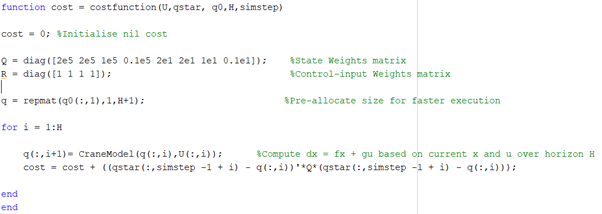
\includegraphics[width=.5\linewidth]{figs/Picture12}
		\caption{A  common 3 axis cartesian FDM 3D printer commonly consisting of 3 actuators}
		\label{figs/Picture12}
	\end{center}
\end{figure}


Give an example in maths notation of a single cost being generated, for one horizon step,
Then give an example of what the cost would be 
Fig. 10:The cost function utilised by fmincon for MPC
The objective cost functions goal was to find such a control force that minimised the error between the end effector position and its desired position at each step in time along its trajectory. This was done by computing the 8xH horizon prediction matrix qH based on the nominal 4xH horizon control matrix U. The cost was then defined as the sum of the squared error between the current and desired states at each point along the trajectory multiplied by the tuning matrix Q. This framework mimics a simple Proportional controller. \\
As we assumed ideal actuators, there was no cost punishment on the actuators.
\subsection*{Constraints and Bounds}
Upper-bound and lower-bound for control forces U based on actuator torque limits.


%%%%%%%%%%%%%%%%%%%%%%%%%%%%%%%%%%%%%%%%%%%
\newpage
\section*{Chapter 4}
\addcontentsline{toc}{section}{Chapter 4}
\section{Simulation}

\subsection{MATLAB functions for Simulated System}

\begin{table}[H]
	\begin{centering}
	\begin{tabular}{ll}
		\textbf{Function Name}               & \textbf{Description}                                                                                                                    \\ \hline
		FKM.m                       &\begin{tabular}[c]{@{}l@{}}    Generates the transformation matrices given joint angle \\ and displacements  \end{tabular}                                                     \\ \hline
		IKM.m                       & \begin{tabular}[c]{@{}l@{}}    Generated the joint angles and displacements given \\ cartesian coordinates. \end{tabular}                                                       \\ \hline
		costvel.m                   & Cost function used for NLMPC.                                                                                                  \\ \hline
		massmatrix.m                & Run the simulation for the nonlinear model using ode4                                                                          \\ \hline
		nonlcon.m                   & Non-linear constraints for the NLMPC                                                                                           \\ \hline
		ode4.m                      & 4th order Runga-Kutta solver                                                                                                   \\ \hline
		TrajectoryGenereration.m    & \begin{tabular}[c]{@{}l@{}} Generates a trajectory as a trapezoidal profile\\ between each waypoint.     \end{tabular}                                                       \\ \hline
		TrajectoryGenerationNEW.m   & \begin{tabular}[c]{@{}l@{}}  Generates a trajectory given a velocity and \\ acceleration constraint while incorporating the blend feature\\ for smooth motion.\end{tabular}    \\ \hline
		RUNLQR.m & \begin{tabular}[c]{@{}l@{}}  Run a script with a set of instructions for LQR\\ control and Feedback linearization to simulate the\\ model given some waypoints. \end{tabular}  \\ \hline
		RUNMPC.m & \begin{tabular}[c]{@{}l@{}} Run a script with a set of instructions for MPC\\ control and Feedback linearization to simulate the\\ model given some waypoints.  \end{tabular}  \\ \hline
		Parameters.m                & Parameters for the constants used in the system.                                                                               \\ \hline
		Parameters\_DH.m            & Parameters used for Denavit Hartenberg convention                                                                              \\ \hline
		controllervel.m             & Setup for NLMPC controller using fmincon.                                                                                      \\ \hline
		plotRobot.m                 & \begin{tabular}[c]{@{}l@{}}  Plotting the animation for the robot following \\the desired trajectory.  \end{tabular}                                                          \\ \hline
		geometricJacobian.m         & Calculation for geometric Jacobian                                                                                             \\ \hline
		skew.m                     & \begin{tabular}[c]{@{}l@{}} takes column vector u of length 3 and returns a matrix $S$ \\ such that $S_v = u \times v$.   \end{tabular}                                                  \\ \hline
		drawFrame.m                 & Draws a frame for plotting                                                                                                     \\ \hline
		mstraj.m                    & Generates a smooth trajectory with blends \\ \hline                                                                                      
	\end{tabular}
\end{centering}
\end{table}

\subsection{Trajectory Generator Applied to Controlled System}

[TODO] We can apply the use of our trajectory generator to produce a path for the LQR CRANE SYSTEM to follow. \\
As an example, the University logo is an excellent example, as it has both sharp edges and smooth curves. 


\begin{figure}[H]
	\begin{center}
		
\includegraphics[width=.5\linewidth]{figs/Picture21}
		\caption{A  common 3 axis cartesian FDM 3D printer commonly consisting of 3 actuators}
		\label{figs/Picture21}
	\end{center}
\end{figure}

 
Fig. 11: University of Newcastle logo
University of Newcastle Logo to be drawn using our printer

\begin{figure}[H]
	\begin{center}
		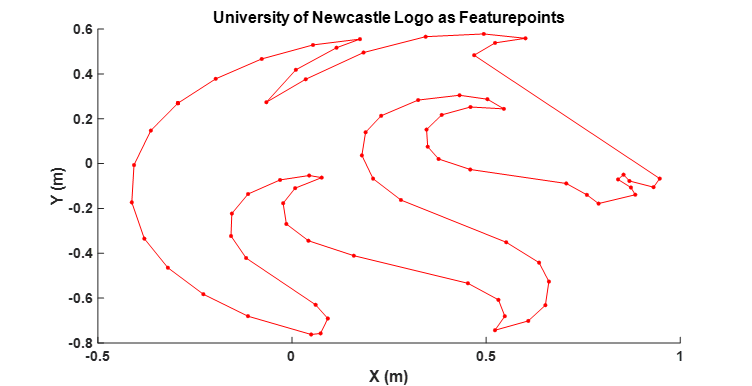
\includegraphics[width=.5\linewidth]{figs/Picture22}
		\caption{A  common 3 axis cartesian FDM 3D printer commonly consisting of 3 actuators}
		\label{figs/Picture22}
	\end{center}
\end{figure}

Fig. 12:Feature points (explain what this is e.g corners, edges) extracted from logo

\begin{figure}[H]
	\begin{center}
		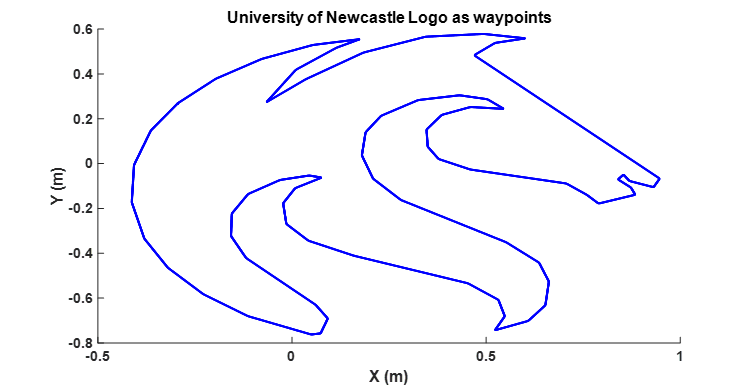
\includegraphics[width=.5\linewidth]{figs/Picture23}
		\caption{A  common 3 axis cartesian FDM 3D printer commonly consisting of 3 actuators}
		\label{figs/Picture23}
	\end{center}
\end{figure}

Fig. 13:Waypoints extracted from logo
Feature points converted to waypoints using trajectory generator

\begin{figure}[H]
	\begin{center}
		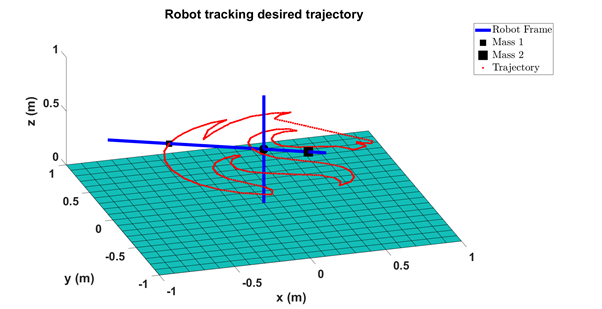
\includegraphics[width=.5\linewidth]{figs/Picture24}
		\caption{A  common 3 axis cartesian FDM 3D printer commonly consisting of 3 actuators}
		\label{figs/Picture24}
	\end{center}
\end{figure}

\section{LQR Tracking Desired Trajectory Test}

[TODO] Write that this is the results from the LQR

\begin{figure}[H]
	\begin{center}
		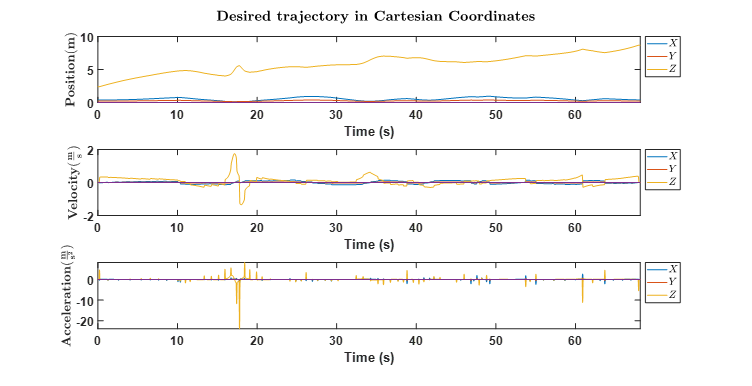
\includegraphics[width=.5\linewidth]{figs/Picture25}
		\caption{A  common 3 axis cartesian FDM 3D printer commonly consisting of 3 actuators}
		\label{figs/Picture25}
	\end{center}
\end{figure}

Fig. 14:The simulated tower crane model tracking the trajectory
What does this image contain? Exlain it like to a blind person ere

\begin{figure}[H]
	\begin{center}
		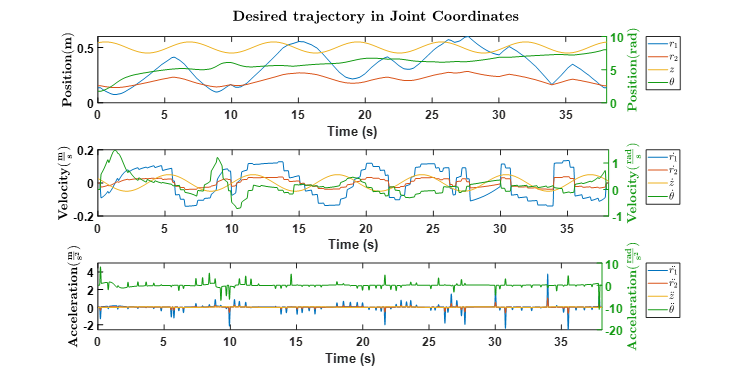
\includegraphics[width=.5\linewidth]{figs/Picture26}
		\caption{A  common 3 axis cartesian FDM 3D printer commonly consisting of 3 actuators}
		\label{figs/Picture26}
	\end{center}
\end{figure}

Fig. 15:The desired trajectory in task space coordinates
Explain this as if to someone who is blind
The trajectory then transforms through inverse kinematics from the cartesian space to the joint space

\begin{figure}[H]
	\begin{center}
		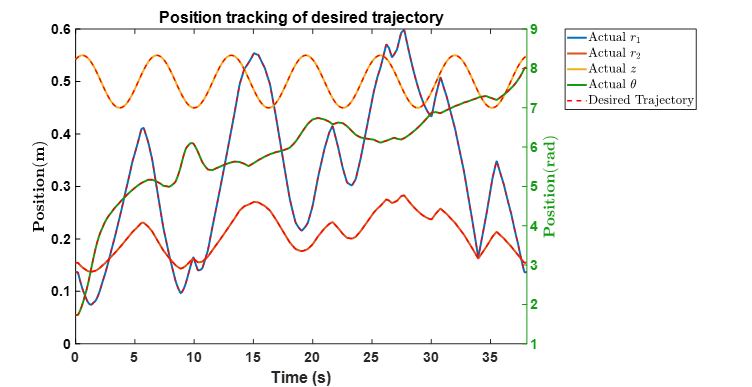
\includegraphics[width=.5\linewidth]{figs/Picture27}
		\caption{A  common 3 axis cartesian FDM 3D printer commonly consisting of 3 actuators}
		\label{figs/Picture27}
	\end{center}
\end{figure}

Fig. 16:The desired trajectory in joint space coordinates

Is this just desired? Or actual? Or both, whats happening in this image?


\section{Using LQR} 

\begin{figure}[H]
	\begin{center}
		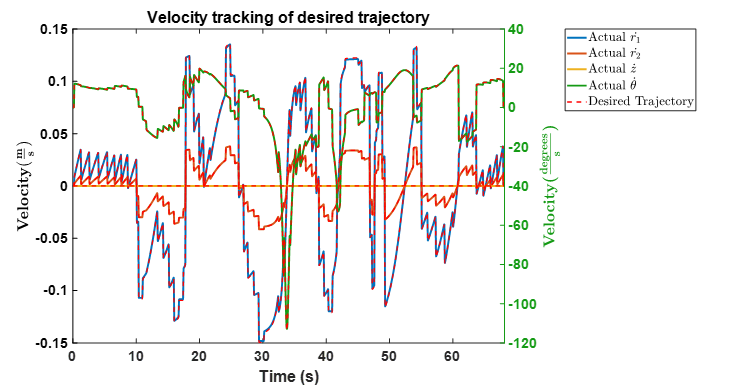
\includegraphics[width=.5\linewidth]{figs/Picture28}
		\caption{A  common 3 axis cartesian FDM 3D printer commonly consisting of 3 actuators}
		\label{figs/Picture28}
	\end{center}
\end{figure}

Fig. 17:Simulated results of the LQR controller tracking a desired trajectory

\begin{figure}[H]
	\begin{center}
		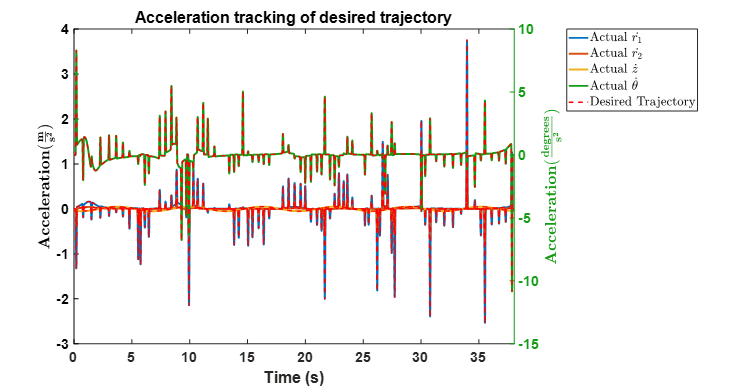
\includegraphics[width=.5\linewidth]{figs/Picture29}
		\caption{A  common 3 axis cartesian FDM 3D printer commonly consisting of 3 actuators}
		\label{figs/Picture29}
	\end{center}
\end{figure}


Fig. 18:Simulated results of the LQR controller tracking a desired trajectory

\begin{figure}[H]
	\begin{center}
		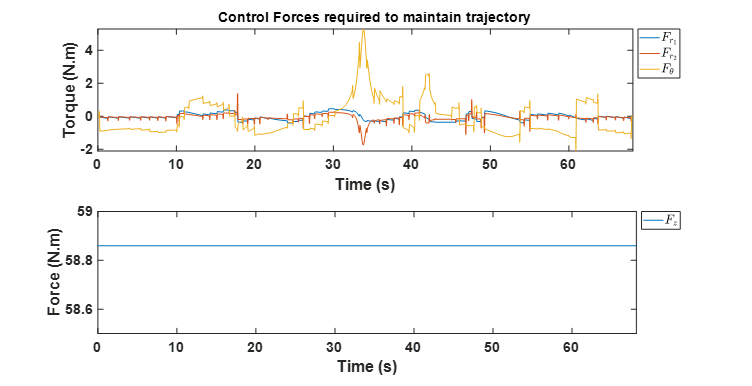
\includegraphics[width=.5\linewidth]{figs/Picture30}
		\caption{A  common 3 axis cartesian FDM 3D printer commonly consisting of 3 actuators}
		\label{figs/Picture30}
	\end{center}
\end{figure}


Fig. 19:Acceleration tracking 

\begin{figure}[H]
	\begin{center}
		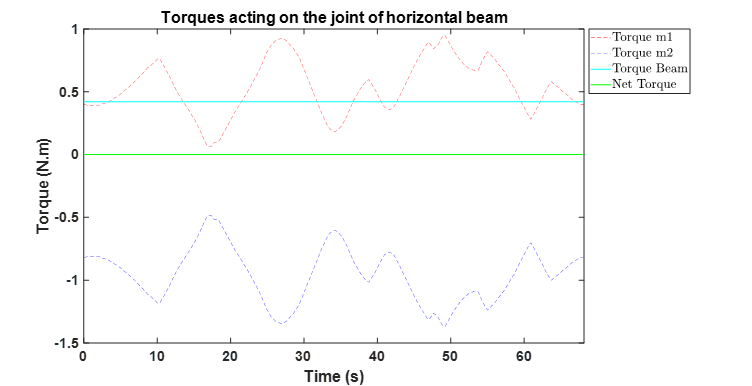
\includegraphics[width=.5\linewidth]{figs/Picture31}
		\caption{A  common 3 axis cartesian FDM 3D printer commonly consisting of 3 actuators}
		\label{figs/Picture31}
	\end{center}
\end{figure}


Fig. 20: Control forces applied by actuators 

\begin{figure}[H]
	\begin{center}
		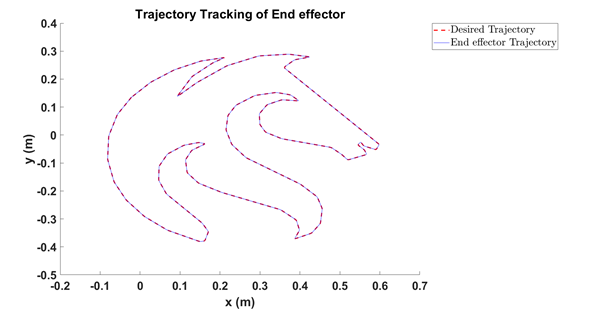
\includegraphics[width=.5\linewidth]{figs/Picture32}
		\caption{A  common 3 axis cartesian FDM 3D printer commonly consisting of 3 actuators}
		\label{figs/Picture32}
	\end{center}
\end{figure}

Fig. 21:Sum of Moments acting on the vertical beam
Note how the sharp the edges of the seahorse is

\begin{figure}[H]
	\begin{center}
		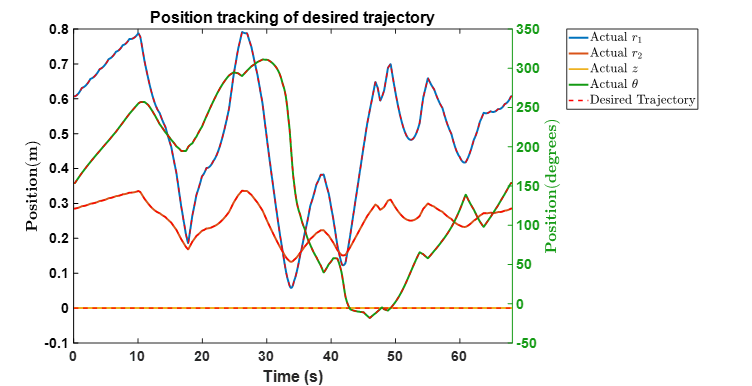
\includegraphics[width=.5\linewidth]{figs/Picture33}
		\caption{A  common 3 axis cartesian FDM 3D printer commonly consisting of 3 actuators}
		\label{figs/Picture33}
	\end{center}
\end{figure}

Fig. 22:Desired trajectory overlaid with end-effector trajectory
Simulation of robot end effector following desired trajected

\section{Using NLMPC}

MPC FORMULATION
[TODO] MPC FORMULATION
MPC RESULTS

\begin{figure}[H]
	\begin{center}
		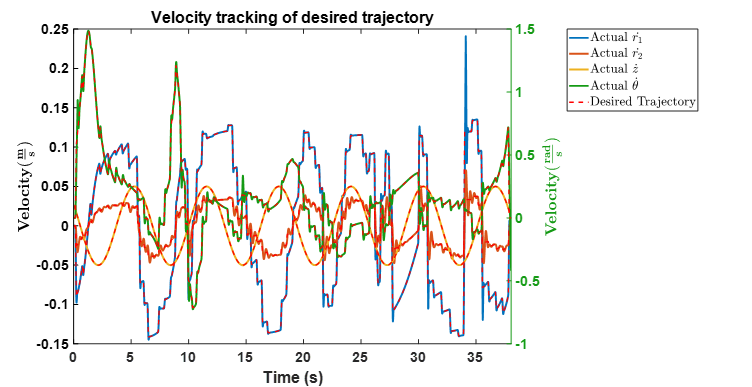
\includegraphics[width=.5\linewidth]{figs/Picture34}
		\caption{A  common 3 axis cartesian FDM 3D printer commonly consisting of 3 actuators}
		\label{figs/Picture34}
	\end{center}
\end{figure}

Fig. 23:position tracking using MPC

\begin{figure}[H]
	\begin{center}
		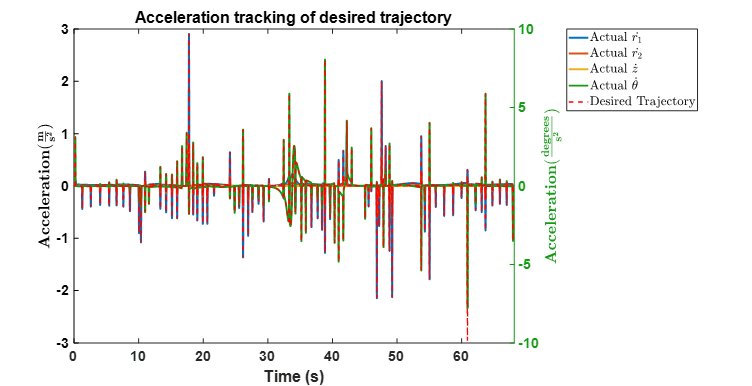
\includegraphics[width=.5\linewidth]{figs/Picture35}
		\caption{A  common 3 axis cartesian FDM 3D printer commonly consisting of 3 actuators}
		\label{figs/Picture35}
	\end{center}
\end{figure}

Fig. 24:velocity tracking using MPC

\begin{figure}[H]
	\begin{center}
		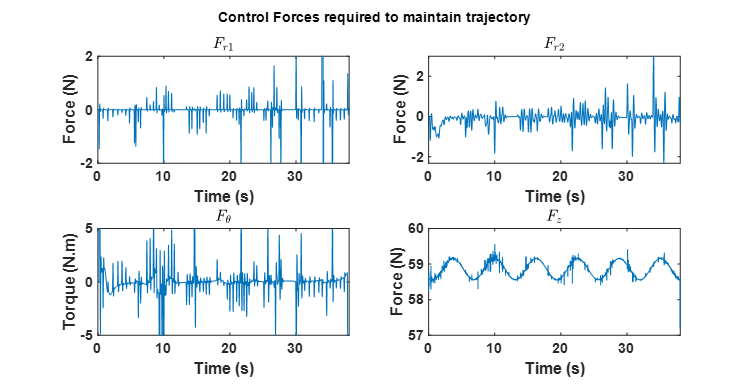
\includegraphics[width=.5\linewidth]{figs/Picture36}
		\caption{A  common 3 axis cartesian FDM 3D printer commonly consisting of 3 actuators}
		\label{figs/Picture36}
	\end{center}
\end{figure}

Fig. 25 Acceleration tracking using MPC

Fig. 26:Control forces demanded by MPC


\section{Discussion}

\subsection{LQR}

Did it work? What do the resulting graphs say?\\
How difficult was it to implement?\\
Was the speed of computation useful for tuning the system?\\
Is this an ideal system for a real system?\\
How robust is it? Is it better than PID control? (electricity costs money and this is optimal)\\
Overall, what have you learned about the use of tragectory generators with respect to LQR\\

\subsection{NLMPC}

Did it work? What do the resulting graphs say?\\
How difficult was it to implement?\\
Was the speed of computation useful for tuning the system? \\
Is this an ideal system for a real system?\\
How robust is it? Is it better than LQR control? (electricity costs money and this is optimal)\\
Was it hard to implement trajectory generation? Why? Why not?\\

\subsection{Comparison}

Chopping and changing MPC is hard

\section{Conclusion}
This is one of the most important parts of the report. In the conclusion section, you should \\
briefly summarise the results,\\
“In this report, a crane model was developed using lagrangian mechanics. Two suitable modern control methods were developed and applied to the system in a coordinated simulation. thing here) was used.\\  
reflect on the work presented,\\
Overall, the system was successful and could be applied to real systems and im going to explain why\\
make recommendations\\
Which control method would you pick, which trajectory method do you suggest, and explain why\\
suggest future work or improvements.\\

If someone were to follow your work, what are the next three steps they would have to take in order to actually make money off this project\\
Be careful with feedback linearization\\
Use robust feedback linearization\\
Make sure observability, in real life you need a nonlinear observer\\


%%%%%%%%%%%%%%%%%%%%%%%%%%%%%%%%
\newpage
\bibliographystyle{harvard} %%ieeetran -- FYP_REFERENCES
\bibliography{References} % This is the .bib file where the bibliography database is stored
%%%%%%%%%%%%%%%%%%%%%%%%%%%%%%
\newpage
\appendix

\section{Appendix A}

\begin{table}[H] \label{tab:physical Characteristics}
	\caption{Definition of symbols}
	\begin{tabular}{lll}
		\textbf{Physical Characteristics}                 & \textbf{Symbology} & \textbf{Units}                              \\ \hline
		Acceleration of gravity                           & g                  & $m/s^2 $     \\
		Distance of nozzle from centre of the beam        &$ r_1 $              & m                                           \\
		Distance of counterweight from centre of the beam & $r_2$               & m                                           \\
		Mass of nozzle                                    & $m_1$               & kg                                          \\
		Mass of Counterweight                             & $m_2 $              & kg                                          \\
		Angular position of the tower                     & $\theta$                  & rad                                         \\
		Generalized coordinates                           & $q$                  & $m,rad$                                     \\
		Generalized velocities                            & $\dot{q}$          & $m/s,m/rad$ \\
		Kinetic Energy                                    & K                  & J                                           \\
		Potential Energy                                  & U                  & J                                           \\
		Lagrangian                                        & L                  & J                                          
	\end{tabular}
\end{table}


\end{document}
